%%%%% SOME OPTIONS %%%%% 
\newcommand{\german}{true} % germanTrue or false --> Switch between german and english headers / titlepage
\newcommand{\coloredTitlePage}{true} % Switch between colored and BW titlepage
\newcommand{\company}{false}
\newcommand{\ECE}{true}
%%%%% Required Settings for the template %%%%%
\input{ECEconfig.sty}
\usepackage{hyperref}

\makeglossaries

\makeatletter
\ctikzset{current arrow color/.initial=black}% create key

\let\old@circ@drawcurrent=\pgf@circ@drawcurrent
\def\pgf@circ@drawcurrent{\old@circ@drawcurrent}

\pgfdeclareshape{currarrow}{
\anchor{center}{
\pgfpointorigin
}
\anchor{tip}{
\pgfpointorigin
    \pgf@circ@res@step = \pgf@circ@Rlen
        \divide \pgf@circ@res@step by 16
\pgf@x  =\pgf@circ@res@step
}
\behindforegroundpath{      

\pgfscope
    \pgf@circ@res@step = \pgf@circ@Rlen
    \divide \pgf@circ@res@step by 16

    \pgfpathmoveto{\pgfpoint{-.7\pgf@circ@res@step}{0pt}}
    \pgfpathlineto{\pgfpoint{-.7\pgf@circ@res@step}{-.8\pgf@circ@res@step}}
    \pgfpathlineto{\pgfpoint{1\pgf@circ@res@step}{0pt}}
    \pgfpathlineto{\pgfpoint{-.7\pgf@circ@res@step}{.8\pgf@circ@res@step}}
    \pgfpathlineto{\pgfpoint{-.7\pgf@circ@res@step}{0pt}}           
    \pgfsetcolor{\pgfkeysvalueof{/tikz/circuitikz/current arrow color}}
    \pgfusepath{draw,fill}

\endpgfscope
}
}
\pgfdeclareshape{flowarrow}{
    \anchor{center}{\pgfpointorigin}
    \anchor{tip}{
    \pgfpointorigin
        \pgf@circ@res@step = \pgf@circ@Rlen
            \divide \pgf@circ@res@step by 16
    \pgf@x  =\pgf@circ@res@step
    }
\behindforegroundpath{
    \pgfscope
        \pgf@circ@res@step = \pgf@circ@Rlen
        \divide \pgf@circ@res@step by 4
        \pgfpathmoveto{\pgfpoint{-\pgf@circ@res@step}{0pt}}
        \pgfpathlineto{\pgfpoint{\pgf@circ@res@step}{0pt}}
        %\pgfsetcolor{\pgfkeysvalueof{/tikz/circuitikz/color}}
  \pgfsetcolor{\pgfkeysvalueof{/tikz/circuitikz/current arrow color}}
        \pgfusepath{draw}
        \pgftransformshift{\pgfpoint{\pgf@circ@res@step}{0pt}}
        \pgfnode{currarrow}{tip}{}{}{\pgfusepath{fill}}
    \endpgfscope
}
}

\makeatletter
\newcommand{\myscope}[2] % #1 = name , #2 = rotation angle
{\draw[thick,rotate=#2] (#1) circle (12pt)
 (#1) ++(-0.35,-0.1) -- ++(0.3,0.3) --++(0,-0.3)-- ++(0.3,0.3) --++(0,-0.3);
}
\newcommand{\costumPicWidth}[0]{
0.8\textwidth
}

\begin{document}
\input{frontmatter/glossaries}
%frontmatter inluding:
%titlepage, abstract, acknowledgments, declaration, toc, lof, lot
\frontmatter
\renewcommand{\thepage}{\Roman{page}}

\input{frontmatter/titlepage}

\tableofcontents
\printglossary
%mainmatter inluding: Parts, chapters, sections, appendicies
\mainmatter
%Hier die verschiedenn tex_Dokumente der Labore einfügen
\chapter{Operationsverstärker Grundschaltungen}
\section{Spannungsfolger mit uA741}
\subsection{Aufgabenstellung}
Die Offsetspannung des Operationsverstärkers ist mit dem Tischmultimeter zu messen, dabei ist mittels eines Potentiometers ein Offsetabgleich vorzunehmen. Danach soll das Gehäuse mit Kältespray abgekühlt werden und die damit verschobene Offsetverschiebung aufzunehmen. 

Die Grenzfrequenz dieser Schaltung ist zu bestimmen und mit einer PSPICE Simulation zu vergleichen. Dabei sollte eine Eingangsspannung mit $V_{PP} = 100 \rm mV$ verwendet werden. 

Der Aussteuerbereich bei einer Eingangsfrequenz von $f=1 \rm kHz$ ist zu bestimmen, dabei sind die Messungen sowohl mit eine Last von $R_{Last} = 2 \rm k\Omega$ als auch ohne Last vorzunehmen. Dafür ist die Amplitude der Eingangsspannung schrittweise zu erhöhen bis eine deutliche Übersteuerung in beiden Halbwellen zu sehen ist. Für diesen Zweck ist die Versorgungsspannung auf $V_{CC} = 10\rm V$ und $V_{EE} = -10 \rm V$ zu verringern. 

Danach ist die negative Versorgungsspannung auf $V_{EE} = -5V$ zu verringern und das daraus resultierende Verhalten zu dokumentieren.

Durch anlegen einer Rechteckspannung ist die Slew Rate des Verstärkers zu bestimmen. Diese ist sowohl mit einem Lastwiderstand von $R_{Last} = 2\rm k\Omega$, als auch mit einer kapazitiven Last von $C_{Last} = 100 \rm nF$ zu bestimmen. 

Durch Kenntnis der maximalen Slew Rate ist nun die sinusförmige Spannung am Eingang anzulegen, welche gerade noch unverzerrt übertragen werden kann. Ausgehend von dieser Spannung ist nun die Frequenz schrittweise zu erhöhen bis eine deutliche Verzerrung zu erkennen ist. 
\begin{figure}[H]
    \centering
    \begin{circuitikz}[]
        \draw (0,0) node[op amp] (opamp) {$\mu A 741$};
        \draw (opamp.up) --++(0,0.5) node[vcc]{$V_{CC}$};
        \draw (opamp.down) --++(0,-0.5) node[vee]{$V_{EE}$};
        \draw (opamp.+) to[short,-o] ++(-2,0) node[left] {$U_{In}$};
        \draw (opamp.out) to[short,-o] ++(3,0) node[right] {$U_{a}$};
        \draw (opamp.-) to[short] ++(-1,0)
            to[short] ++(0,2)
            to[short] ++(6,0)
            to[short,-*] ++(0,-2.5);
        \draw (0.3,0.3) to[short] ++(0,0.5)
            to[short] ++(2.5,0)
            to[short] (2.8,-1)
            to[pR, name=offsetPoti] ++(-2,0)
            to[short] ++(-0.5,0)
            to[short] (0.3,-0.3);
        \draw (offsetPoti.wiper) node[vee]{$V_{EE}$};
        
        \end{circuitikz}
    \caption{Spannungsfolger mit Offsettrimmer}
    \label{fig:Spannungsfolger_Schaltung}
 \end{figure}

\subsection{Messaufbau}
Um alle gegebene Aufgabenstellungen erfüllen zu können, wurde die Schaltung mit zwei verschiedenen Messbeschaltungen versehen. 

zur Bestimmung der Offsetspannung wurde der Eingang der Schaltung mit Masse verbunden. Danach wurde die Ausgangsspannung mit dem Tischmultimeter gemessen und aufgezeichnet.

Im zweiten Aufbau wurde der Eingang mit einem Signagenerator betrieben und Ein- und Ausgang mit dem Oszilloskop gemessen. Für bestimmte Messungen wurde der Ausgang zusätzlich mit einem $R_{Last} = 2k\Omega$ und einem $C_{Last} = 100nF$ belastet.
\begin{figure}[H]
    \centering
    \begin{circuitikz}[]
        \draw (0,0) node[op amp] (opamp) {$\mu A 741$};
        \draw (opamp.up) --++(0,0.5) node[vcc]{$V_{CC}$};
        \draw (opamp.down) --++(0,-0.5) node[vee]{$V_{EE}$};
        \draw (opamp.+) to[short,-o] ++(-1,0) 
            %%Einfügen der Messschaltung
            to[short,o-o] ++(0,-1) node[ground] {};
        \draw (opamp.out) to[short,-o] ++(3,0)
            %Einfügen der Messchaltung
            to[voltmeter,o-o] ++(0,-2) node[ground]{};
        \draw (opamp.-) to[short] ++(-1,0)
            to[short] ++(0,2)
            to[short] ++(6,0)
            to[short,-*] ++(0,-2.5);
        \draw (0.3,0.3) to[short] ++(0,0.5)
            to[short] ++(2.5,0)
            to[short] (2.8,-1)
            to[pR, name=offsetPoti] ++(-2,0)
            to[short] ++(-0.5,0)
            to[short] (0.3,-0.3);
        \draw (offsetPoti.wiper) node[vee]{$V_{EE}$};
        
        \end{circuitikz}
    \caption{Spannungsfolger, Messaufbau zur Offsetbestimmung, $V_{CC} = 15\rm V$, $V_{EE} = -15\rm V$}
    \label{fig:Spannungsfolger_Messaufbau_Offset}
 \end{figure}

\begin{figure}[H]
    \centering
    \begin{circuitikz}[]
        \draw (0,0) node[op amp] (opamp) {$\mu A 741$};
        \draw (opamp.up) --++(0,0.5) node[vcc]{$V_{CC}$};
        \draw (opamp.down) --++(0,-0.5) node[vee]{$V_{EE}$};
        \draw (opamp.+) to[short,-o] ++(-1,0) 
            %%Einfügen der Messschaltung
            to[sV=CH1, color=white, name=S1,o-o] ++(0,-2) node[ground] {}
            to[short,o-] ++(-2,0)
            to[sV] ++(0,2)
            to[short,-o] ++(2,0);
        \draw (opamp.out) to[short,-o] ++(3,0)
            %Einfügen der Messchaltung
            to[sV=CH2, color=white, name=S2,o-o] ++(0,-2) node[ground]{};
        \draw (opamp.-) to[short] ++(-1,0)
            to[short] ++(0,2)
            to[short] ++(6,0)
            to[short,-*] ++(0,-2.5);
        \draw (0.3,0.3) to[short] ++(0,0.5)
            to[short] ++(2.5,0)
            to[short] (2.8,-1)
            to[pR, name=offsetPoti] ++(-2,0)
            to[short] ++(-0.5,0)
            to[short] (0.3,-0.3);
        \draw (offsetPoti.wiper) node[vee]{$V_{EE}$};
        \myscope{S1}{0}
        \myscope{S2}{0}
        \end{circuitikz}
    \caption{Spannungsfolger, Messaufbau zur Bestimmung des zeitlichen Verhaltens}
    \label{fig:Spannungsfolger_Messaufbau_Offset}
 \end{figure}

\subsection{Messergebnisse}
Bei der Messung der Offsetspannung ohne dem Einbau eines Trimmers zur Anpassung wurde eine Spannung von $V_{IO} = 1,792 mV$ gemessen. Diese Messung konnte mittels des Datenblattes verifiziert werden. Laut diesem sollte die Offsetspannung zwischen 1mV und 5mV liegen.\cite[6]{ti:ua741}

Nun wurde der mithilfe des Trimmers auf eine Offsetspannung von $V_{IO Trimm} = 160 \mu V$ verringert. Durch abkühlen mit einem Kältspray wurde zunächst nur wenig Änderung am Ausgang beobachtet, jedoch erhöhte sich der Offset nach einigen Sekunden signifikant, bis er ein Maximum von $V_{IO} = 2,2mV$ erreichte. 

Wie in Abbildung \ref{fig:Bode_Folger_ua741} zu sehen ist, beträgt die Grenzfrequenz der Schaltung $f_C=850KHz$. Das ist ungefähr 150KHz weniger als durch Angaben im Datenblatt, sowie der Simulation zu erwarten wäre. Die Begründung für dieses Phänomen liegt wahrscheinlich in der kapazitiven Belastung der Schaltung durch das Messequipment, sowie die kleinen Leckströme die über die Kapazitäten des Steckbretts fließen und der nicht-idealen Entkopplung der Schaltung durch den Aufbau am Steckbrett. 

\begin{figure}[H]
    \centering
    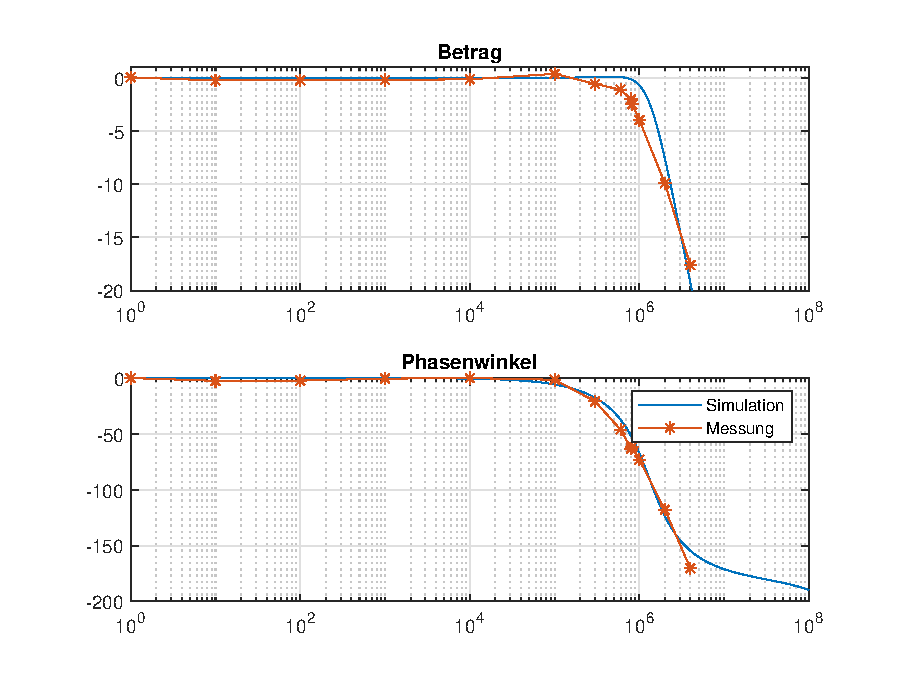
\includegraphics[width=0.8\textwidth]{Lab_1/Plots/Folger.eps}
    \caption{Bodediagramm der Folgerschaltung, $V_{inPP}=100mV$, $V_{CC}=-V_{EE}=15V$}
    \label{fig:Bode_Folger_ua741}
\end{figure}

\begin{table}[H]
\centering
\caption{Aussteuerbereich,  $V_{CC}=-V_{EE}=10V$}
\label{tab:Clip_Folger_ua741}
\begin{tabular}{|l|l|}
\hline
unbelastet       & $R_{Last} = 2k\Omega$ \\ \hline
$V_{CC} - 0,49V$ & $V_{CC} - 1,23V$      \\ \hline
$V_{EE} + 1,67V$ & $V_{EE} + 2,39V$      \\ \hline
\end{tabular}
\end{table}

\begin{figure}[H]
    \centering
    \includegraphics[width=0.8\textwidth]{Lab_1/Messungen/Folger/uberst-schw3.png}
    \caption{Aussteuerbereich $uA741$, $CH_{Ref}: R_{Last} = inf$, $CH_{2}: R_{Last} = 2k\Omega$}
    \label{fig:my_label}
\end{figure}
\begin{figure}[H]
    \centering
    \includegraphics[width=0.8\textwidth]{Lab_1/Messungen/Folger/uberst-schw5.png}
    \caption{Aussteuerbereich Detailansicht $uA741$, $CH_{Ref}: R_{Last} = inf$, $CH_{2}: R_{Last} = 2k\Omega$}
    \label{fig:my_label}
\end{figure}

\begin{figure}[H]
    \centering
    \includegraphics[width=0.8\textwidth]{Lab_1/Messungen/Folger/scope_5.png}
    \caption{Aussteuerbereich $uA741$, $CH_{Ref}: R_{Last} = inf$, $CH_{2}: R_{Last} = 2k\Omega$, $V_{CC} = 10V$, $V_{EE} = -5V$}
    \label{fig:my_label}
\end{figure}

\begin{figure}[H]
    \centering
    \includegraphics[width=0.8\textwidth]{Lab_1/Messungen/Folger/uberst-schw13.png}
    \caption{Slew Rate $uA741$, $CH_{Ref}$}
    \label{fig:my_label}
\end{figure}

\section{Nicht invertierender Verstärker}
\subsection{Aufgabenstellung}
Es ist die Schaltung aus Abbildung \ref{fig:niinv_Verst_Schaltung} aufzubauen und mit  einer Verstärkung von $\nu=+10$ und $\nu = +101$ auszulegen. Dabei ist die Frequenz zu finden bei welcher der Verstärker das Signal aufgrund der Slew Rate verzerrt. 

Es sind die Frequenzgänge mit den beiden Verstärkungen aufzunehmen und mit der Verstärkung des geschlossenen Kreises zu vergleichen.

Die Kurve $U_a = f(U_e)$ der Schaltung mit $\nu=10$ ist mittels des X-Y-Betriebs des Oszilloskops aufzuzeichnen.

Das Verhalten bei rechteckförmigen Eingangsspannungen ist aufzunehmen.
\begin{figure}[H]
    \centering
    \begin{circuitikz}[]
        \draw (0,0) node[op amp,yscale=-1] (opamp) {\scalebox{1}[-1]{$\mu A 741$}};
        \draw (opamp.down) --++(0,0.5) node[vcc]{$V_{CC}$};
        \draw (opamp.up) --++(0,-0.5) node[vee]{$V_{EE}$};
        
        \draw (opamp.+) to[short,-o] ++(-2,0) node[left] {$U_{in}$};
        \draw (opamp.-) to[short] ++(-0.5,0)
            to[short] ++(0,-2.5)
            to[R=$R_1$] ++(0,-1.5) node[ground]{};
        \draw (opamp.out) to[short,-o] ++(2,0) node[right] {$U_a$};
        \draw (2,0) to[short,*-] ++(0,-2.5)
            to[R=$R_2$,-*] (-1.7,-2.5);
        \end{circuitikz}
    \caption{Nicht invertierender Verstärker}
    \label{fig:niinv_Verst_Schaltung}
 \end{figure}


\subsection{Auslegung der Schaltung}
\subsubsection{Verstärkung 10}
Zur Auslegung dieser Schaltung wurde zuerst ein Widerstand ausgewählt, damit wurde dann der Zweite berechnet.

\begin{align}
    \nu &= 1+ \frac{R_2}{R_1}\\
    R_2 &= 2k\Omega\\
    R_1 = R_2(\nu - 1) &= 18 k\Omega
\end{align}

\subsubsection{Verstärkung 101}
Zur Auslegung dieser Schaltung wurde zuerst ein Widerstand ausgewählt, damit wurde dann der Zweite berechnet.

\begin{align}
    \nu &= 1+ \frac{R_2}{R_1}\\
    R_2 &= 1k\Omega\\
    R_1 = R_2(\nu - 1) &= 100 k\Omega
\end{align}

\subsection{Messaufbau}
Zur Aufnahme aller Messungen wurde sowohl die Ein- als auch die Ausgangsspannung mit dem Oszilloskop aufgenommen. Die Eingangsspannung wurde mit einem Signalgenerator erzeugt, dieser war im High-Z Modus. 
\begin{figure}[H]
    \centering
    \begin{circuitikz}[]
        \draw (0,0) node[op amp,yscale=-1] (opamp) {\scalebox{1}[-1]{$\mu A 741$}};
        \draw (opamp.down) --++(0,0.5) node[vcc]{$V_{CC}$};
        \draw (opamp.up) --++(0,-0.5) node[vee]{$V_{EE}$};
        
        \draw (opamp.-) to[short] ++(-0.5,0)
            to[short] ++(0,-2.5)
            to[R=$R_1$] ++(0,-1.5) node[ground]{};
        
        \draw (opamp.out) to[short,-o] ++(3,0)
            %Einfügen der Messchaltung
            to[sV=CH2, color=white, name=S2,o-o] ++(0,-2) node[ground]{};
        \draw (opamp.+) to[short,-o] ++(-2,0) 
            %%Einfügen der Messschaltung
            to[sV=CH1, color=white, name=S1,o-o] ++(0,-2) node[ground] {}
            to[short,o-] ++(-2,0)
            to[sV] ++(0,2)
            to[short,-o] ++(2,0);        
        \draw (2,0) to[short,*-] ++(0,-2.5)
            to[R=$R_2$,-*] (-1.7,-2.5);
            
        \myscope{S1}{0}
        \myscope{S2}{0}

        \end{circuitikz}
    \caption{Nicht invertierender Verstärker, Messaufbau}
    \label{fig:niinv_Verst_Schaltung_Messaufbau}
 \end{figure}


\subsection{Messergebnisse}
Wie in Abbildung \ref{fig:bode_niinv} zu erkennen ist, die Grenzfrequenz der Schaltung mit der höheren Verstärkung niedriger ist. Anhand des Gain-Bandwidth Produktes ist dieses Ergebnis nachvollziehbar. Es wurden keine signifikanten Abweichungen der Messungen von den Simulationen gefunden. 
\begin{figure}[H]
    \centering
    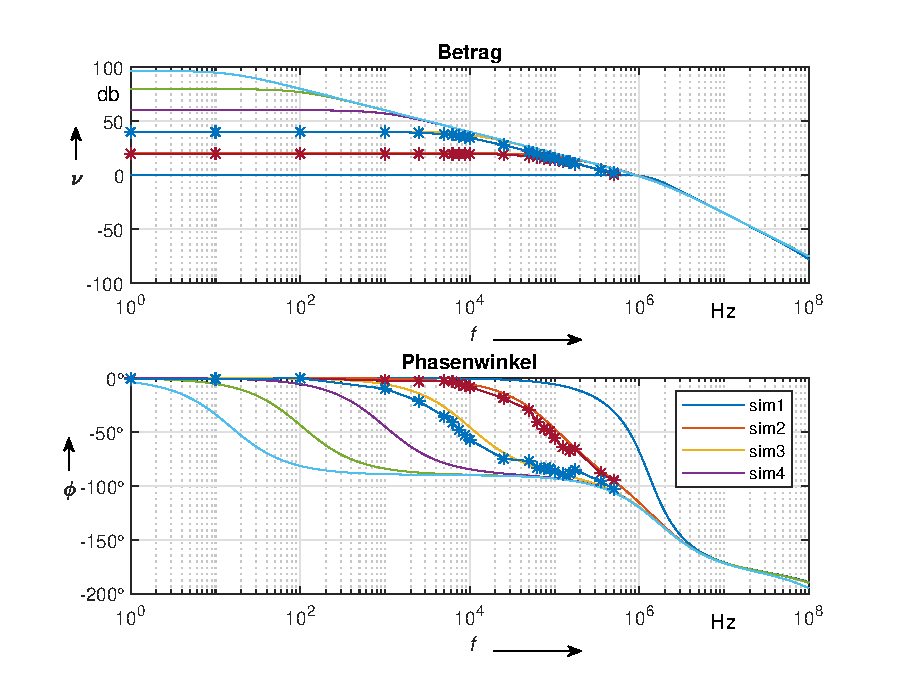
\includegraphics[width=\costumPicWidth]{Lab_1/Plots/niinv_verst.eps}
    \caption{Bodediagramm nicht invertierender Verstärker}
    \label{fig:bode_niinv}
\end{figure}

\begin{figure}[H]
    \centering
    \includegraphics[width=\costumPicWidth]{Lab_1/Messungen/niinv_verst/xy_ohne_uebersteuern_1.png}
    \caption{$U_a = f(U_e)$ im XY Betrieb des Oszilloskops, ohne Übersteuern des Verstärkers }
    \label{fig:niinv_ohne_Uebersteuern}
\end{figure}

\begin{figure}[H]
    \centering
    \includegraphics[width=\costumPicWidth]{Lab_1/Messungen/niinv_verst/xy_mit_uebersteuern_1.png}
    \caption{$U_a = f(U_e)$ im XY Betrieb des Oszilloskops, ohne Übersteuern des Verstärkers}
    \label{fig:niinv_mit_Uebersteuern}
\end{figure}
An der positiven Steigung der Geraden in Abbildung \ref{fig:niinv_mit_Uebersteuern} und \ref{fig:niinv_ohne_Uebersteuern} sieht man dass die Schaltung das Eingangssignal nicht invertiert.

Bei negativer Eingangsspannung fließt eine Spannung in den Eingangspin des Verstärkers, bei positiver Spannung aus dem Pin heraus. 
\begin{figure}[H]
    \centering
    \includegraphics[width=\costumPicWidth]{Lab_1/Messungen/niinv_verst/square.png}
    \caption{Rechteckige Eingangsspannung}
    \label{fig:niinv_rechteck}
\end{figure}

\subsection{Ausarbeitungen}
Der Eingangswiderstand dieser Schaltung wäre bei einem idealen OPamp unendlich groß. Bei dieser Schaltung wird (bei weitem :D) kein idealer Operationsverstärker verwendet, das heißt der Eingangswiderstand der Schaltung entsrpicht dem Eingangswiderstand des nicht-invertierenden Pins des Verstärkers. Dieser ist zwar groß, aber nicht unendlich groß. Um einen definierten Eingagswiderstand zu erhalten, müsste ein paralleler Widerstand (z.B. $R_{IN}=50\Omega$) eingesetzt werden. Der dazu parallele Eingangswiderstandes des Operationsverstärkers wegen seine Größe in den allermeisten Fällen vernachlässigt werden.

\section{Invertierender Verstärker}
\subsection{Aufgabenstellung}
Die Schaltung aus Abbildung \ref{fig:inv_verst_Schaltung} ist für eine Verstärkung $\nu = -10$ auszulegen und auf dem Steckbrett aufzubauen. 

Es ist zu dokumentieren was am virtuellen Nullpunkt der Schaltung bei Übersteuerung des Ausgangs passiert. Diese Messung ist bei einer Frequenz von $f=1kHz$ durchzuführen. 

Mittels des XY-Betriebs ist zu zeigen, in welche Richtung der Strom am OPamp Ausgangspin fließt bei positiven und negativen Ausgangsspannungen. 
\begin{figure}[H]
    \centering
    \begin{circuitikz}[]
        %%Verstärker und Versorgung
        \draw (0,0) node[op amp] (opamp) {$\mu A 741$};
        \draw (opamp.up) --++(0,0.5) node[vcc]{$V_{CC}$};
        \draw (opamp.down) --++(0,-0.5) node[vee]{$V_{EE}$};
        
        \draw (opamp.+) to[short] ++(-0.25,0)
            to[short] ++(0,-0.25) node[ground] {};
        
        \draw (opamp.-) to[short] (-2,0.5)
            to[R=$R_1$,*-o] ++(-2,0) node[left] {$U_{in}$};
        \draw (-2,0.5) to[short] ++(0,2)
            to[R=$R_2$] ++(4,0)
            to[short,-*] ++(0,-2.5);
        \draw (opamp.out) to[short,-o] ++(2,0) node[right] {$U_a$};
        \end{circuitikz}
    \caption{Invertierender Verstärker}
    \label{fig:inv_verst_Schaltung}
 \end{figure}

\subsection{Messaufbau}
\begin{figure}[H]
    \centering
    \begin{circuitikz}[]
        \draw (0,0) node[op amp,yscale=-1] (opamp) {\scalebox{1}[-1]{$\mu A 741$}};
        \draw (opamp.down) --++(0,0.5) node[vcc]{$V_{CC}$};
        \draw (opamp.up) --++(0,-0.5) node[vee]{$V_{EE}$};
        
        \draw (opamp.-) to[short] ++(-0.5,0)
            to[short] ++(0,-2.5)
            to[R=$R_1$] ++(0,-1.5) node[ground]{};
        
        \draw (opamp.out) to[short,-o] ++(3,0)
            %Einfügen der Messchaltung
            to[sV=CH2, color=white, name=S2,o-o] ++(0,-2) node[ground]{};
        \draw (opamp.+) to[short,-o] ++(-2,0) 
            %%Einfügen der Messschaltung
            to[sV=CH1, color=white, name=S1,o-o] ++(0,-2) node[ground] {}
            to[short,o-] ++(-2,0)
            to[sV] ++(0,2)
            to[short,-o] ++(2,0);        
        \draw (2,0) to[short,*-] ++(0,-2.5)
            to[R=$R_2$,-*] (-1.7,-2.5);
            
        \myscope{S1}{0}
        \myscope{S2}{0}

        \end{circuitikz}
    \caption{Nicht invertierender Verstärker, Messaufbau}
    \label{fig:niinv_Verst_Schaltung_Messaufbau}
 \end{figure}

%%tudu

\subsection{Messergebnisse}

\subsection{Ausarbeitungen}
Der Eingangswiderstand dieser Schaltung ist $R_1$. Da beim OPamp im Idealfall an beiden Eingangspins die gleiche Spannung anliegen soll, liegt am virtuellen Nullpunkt das GND Potential an. Daraus ergibt sich, dass $R_1$ der Eingangswiedersatnd der Schaltung ist.



\section{Addierschaltung}
\subsection{Aufgabenstellung}
Die Schaltung aus dem vorherigen Kapitel ist mit einem weitern Eingang zu erweitern. Danach sind zwei verschiedene Wechselspannungen anzulegen. Eine davon sollte einen Gleichspannungsoffset aufweisen. 
\begin{figure}[H]
    \centering
    \begin{circuitikz}[]
        %%Verstärker und Versorgung
        \draw (0,0) node[op amp] (opamp) {$\mu A 741$};
        \draw (opamp.up) --++(0,0.5) node[vcc]{$V_{CC}$};
        \draw (opamp.down) --++(0,-0.5) node[vee]{$V_{EE}$};
        
        \draw (opamp.+) to[short] ++(-0.25,0)
            to[short] ++(0,-0.25) node[ground] {};
        
        \draw (opamp.-) to[short] (-2,0.5)
            to[R=$R_1$,*-o] ++(-2,0) node[left] {$U_{in1}$};
        \draw (-2,2.5) to[R=$R_2$,*-o] ++(-2,0) node[left] {$U_{in2}$};
        \draw (-2,0.5) to[short] ++(0,2)
            to[R=$R_{ref}$] ++(4,0)
            to[short,-*] ++(0,-2.5);
        \draw (opamp.out) to[short,-o] ++(2,0) node[right] {$U_a$};
        \end{circuitikz}
    \caption{Addierschaltung}
    \label{fig:Addierschaltung}
 \end{figure}


\subsection{Messaufbau}
Zur Aufname aller Messungen wurde ein anderer Signalgenerator als im Labor vorhanden war. Ich habe in dieser Laborübung meinen eigenen mitgebracht. Dieser hat den Vorteil, dass er zwei synchronisierte Ausgänge besitzt. Alle Ein- und Ausgänge wurden mit dem Oszilloskop aufgenommen
\begin{figure}[H]
    \centering
    \begin{circuitikz}[]
        \draw (0,0) node[op amp,yscale=-1] (opamp) {\scalebox{1}[-1]{$\mu A 741$}};
        \draw (opamp.down) --++(0,0.5) node[vcc]{$V_{CC}$};
        \draw (opamp.up) --++(0,-0.5) node[vee]{$V_{EE}$};
        
        \draw (opamp.-) to[short] ++(-0.5,0)
            to[short] ++(0,-2.5)
            to[R=$R_1$] ++(0,-1.5) node[ground]{};
        
        \draw (opamp.out) to[short,-o] ++(3,0)
            %Einfügen der Messchaltung
            to[sV=CH2, color=white, name=S2,o-o] ++(0,-2) node[ground]{};
        \draw (opamp.+) to[short,-o] ++(-2,0) 
            %%Einfügen der Messschaltung
            to[sV=CH1, color=white, name=S1,o-o] ++(0,-2) node[ground] {}
            to[short,o-] ++(-2,0)
            to[sV] ++(0,2)
            to[short,-o] ++(2,0);        
        \draw (2,0) to[short,*-] ++(0,-2.5)
            to[R=$R_2$,-*] (-1.7,-2.5);
            
        \myscope{S1}{0}
        \myscope{S2}{0}

        \end{circuitikz}
    \caption{Nicht invertierender Verstärker, Messaufbau}
    \label{fig:niinv_Verst_Schaltung_Messaufbau}
 \end{figure}


\subsection{Messergebnisse}
Zur besseren Darstellung der Addition wurden hier Sinusspannungen mit zwei verschiedenen Frequenzen angelegt. Das Ergebnis entsprach den Erwartungen. 
\begin{figure}[H]
    \centering
    \includegraphics[width=\costumPicWidth]{Lab_1/Messungen/Addierer/scope_25.png}
    \caption{Addition zweier Sinusspannungen}
    \label{fig:Addierschaltung_Ergebnis}
\end{figure}

\section{Geräteverzeichnis}
\begin{table}[H]
\centering
\caption{Geräteverzeichnis 1. Übung}
\label{tab:Gerteverzeichnis}
\begin{tabular}{|
>{\columncolor[HTML]{C0C0C0}}l |l|l|l|}
\hline
Gerät           & \cellcolor[HTML]{C0C0C0}Hersteller & \cellcolor[HTML]{C0C0C0}Bezeichnung & \cellcolor[HTML]{C0C0C0}Seriennummer \\ \hline
Multimeter      & Agilent                            & 34450A                              & 9949728                              \\ \hline
Netzteil        & TTI                                & PL303QMD                            & 9949264                              \\ \hline
Signalgenerator & Keysight                           & 33500B Series                       & 9949719                              \\ \hline
Oszilloskop     & Keysight                           & DSO-X 3014T                         & 9949710                              \\ \hline
\end{tabular}
\end{table}

\chapter{Grundschaltungen mit Frequenzgangbeeinflussung}
\section{Spannungsfolger mit LM358}
\subsection{Aufgabenstellung}
Die Schaltung aus Abbildung \ref{fig:Spannungsfolger_LM358_Schaltung} ist auf einem Steckbrett aufzubauen. Danach ist der Verstärker in die negative Versorgungsspannnung zu übersteuern. Dieses Verhalten ist aufzuzeichnen. 
\begin{figure}[H]
    \centering
    \begin{circuitikz}[]
        \draw (0,0) node[op amp] (opamp) {$LM358$};
        \draw (opamp.up) --++(0,0.5) node[vcc]{$V_{CC}$};
        \draw (opamp.down) --++(0,-0.5) node[vee]{$V_{EE}$};
        \draw (opamp.+) to[short,-o] ++(-2,0) node[left] {$U_{In}$};
        \draw (opamp.out) to[short,-o] ++(2,0) node[right] {$U_{a}$};
        \draw (opamp.-) to[short] ++(-1,0)
            to[short] ++(0,2)
            to[short] ++(4,0)
            to[short,-*] ++(0,-2.5);
        \end{circuitikz}
    \caption{Spannungsfolger mit LM358}
    \label{fig:Spannungsfolger_LM358_Schaltung}
 \end{figure}

\subsection{Messaufbau}
Zur Messung der oben genannten Schaltung wurde die Schaltung mit $V_{CC} = 10V$ und $V_{EE} = -7V$ versorgt. Da das Verhalten bei Übersteuerung gezeigt werden sollte und der verwendete Signalgenerator eine maximale $V_{PP} = 20V$ bereitstellen kann, musste hier eine geringere Versorgungspannung als bei vorherigen Messaufbauten verwendet werden
\begin{figure}[H]
    \centering
    \begin{circuitikz}[]
        \draw (0,0) node[op amp] (opamp) {$LM358$};
        \draw (opamp.up) --++(0,0.5) node[vcc]{$V_{CC}$};
        \draw (opamp.down) --++(0,-0.5) node[vee]{$V_{EE}$};
        \draw (opamp.+) to[short,-o] ++(-1,0) 
            %%Einfügen der Messschaltung
            to[sV=CH1, color=white, name=S1,o-o] ++(0,-2) node[ground] {}
            to[short,o-] ++(-2,0)
            to[sV] ++(0,2)
            to[short,-o] ++(2,0);
        \draw (opamp.out) to[short,-o] ++(2,0)
            %Einfügen der Messchaltung
            to[sV=CH2, color=white, name=S2,o-o] ++(0,-2) node[ground]{};
        \draw (opamp.-) to[short] ++(-1,0)
            to[short] ++(0,2)
            to[short] ++(4,0)
            to[short,-*] ++(0,-2.5);
        \myscope{S1}{0}
        \myscope{S2}{0}
        \end{circuitikz}
    \caption{Spannungsfolger mit LM358, Messaufbau zur Bestimmung des zeitlichen Verhaltens}
    \label{fig:Spannungsfolger_LM358_Messaufbau_Offset}
 \end{figure}

\subsection{Interpretation der Messergebnisse}
Der LM358 zeigt bei Aussteurung über den negatigen Gleichtaktaussteuerbereich eine sogenannte Phasenumkehr. Bei der Messung welche in Abbildung \ref{fig:LM358_Phasenumkehr} dargestellt ist, ist gut zu sehen, dass bei Aussteuerung über der Übersteuerung das Signal nicht einfach geklippt wird, sondern eine Phasenumkehr stattfindet. Das heißt konkret, dass in diesem Fall die positive, statt der negativen Versorgungspannung anliegt. 
\begin{figure}[H]
    \centering
    \includegraphics[width = \costumPicWidth]{Lab_2/Messungen/Follower/scope_35.png}
    \caption{LM358 Phasenumkehr bei negativer Übersteuerung}
    \label{fig:LM358_Phasenumkehr}
\end{figure}

%%%%%%%%%%%%%%%%%%%%%%%%%%%%%%%%%%%%%%%%%%%%%%%%%%%%%%%%%%%%%%%%%%%%%%%%%%%%%%%%%%%%%%%%%%%%%%%%%%%%%%%%%%%%%%%%%%%%%%%%%%%%%%
\section{Tiefpass erster Ordnung mit LM358}
\subsection{Aufgabenstellung}
Die in Abbildung \ref{fig:aktiver_Tiefpass_LM358_Schaltung} dargestellte Tiefpassschaltung ist auf eine $f_g=1kHz$ und eine Verstärkung im Durchlassbereich von $\nu = -10$ auszulegen. Die Schaltung ist auf dem Steckbrett aufzubauen.

Danach sind die Grenzfrequenz und die Verstärkung, das Verhalten bei nicht-sinusförmigen Eingangsspannungen und ein Bodediagramm messtechnisch zu erfassen. 
\begin{figure}[H]
    \centering
    \scalebox{0.75}{
    \begin{circuitikz}[]
        \draw (-8.5,0.5) node[inst amp ra](instamp){AD627};
        \draw (instamp.ra+) to[R=$R_4$] (instamp.ra-);
        \draw (instamp.-) to[R=$R_3$] ++(0,2) node[ground, yscale=-1]{};
        \draw (instamp.-) to[short,*-] ++(-2,0) to[C=$C_3$] ++(0,2) node[ground, yscale=-1]{};
        \draw (instamp.-) to[short,*-] ++(-2,0) to[C=$C_1$] ++(-2,0) to[R=$R_1$,-o] ++(-2,0) node[left]{Grün};

        \draw (instamp.+) to[R=$R_5$] ++(0,-2) node[ground]{};
        \draw (instamp.+) to[short,*-] ++(-2,0) to[C=$C_5$] ++(0,-2) node[ground]{};
        \draw (instamp.+) to[short,*-] ++(-2,0) to[C=$C_2$] ++(-2,0) to[R=$R_2$,-o] ++(-2,0) node[left]{Rot};

        \draw (instamp.-) to[short,*-] ++(-2,0) to[C=$C_4$,*-*] ++(0,-2.85);
        
        \draw (-16,-3) node[left] {Gelb} to[short,o-]++(1,0) to[short]++(0,-1) node[ground]{};
        
        \draw (instamp.refv down) to[short] ++(0,-1) node[ground]{};
        
        \draw (0,0) node[op amp,yscale=-1] (opamp) {\scalebox{1}[-1]{$AD823$}};
        \draw (opamp.down) --++(0,0.5) node[vcc]{$V_{CC}$};
        \draw (opamp.up) --++(0,-0.5) node[vee]{$V_{EE}$};
        
        \draw (opamp.+) to[short, -*] ++(-2,0)
            to[C=$C_7$] ++(0,-2) node[ground]{};
        \draw (opamp.+) to[short, -*] ++(-2,0)
            to[R=$R_7$] ++(-2,0)
            to[R=$R_6$] ++(-2,0);
        \draw (-5.25,0.5) to[short,*-] ++(0,2)
            to[C=$C_6$] ++(7.445,0)
            to[short] ++(0,-2.5)
            to[short] (opamp.out);
        \draw (opamp.out) to[short,-*] ++(1,0)
            to[R=$R_9$,-*] ++(0,-3)
            to[R=$R_8$] ++(0,-2) node[ground]{};
        \draw (2.2,-3) to[short] ++(-4,0)
            to[short] ++(0,2.5)
            to[short] (opamp.-);
        \draw (opamp.out) to[short,-o] ++(2,0) node[right] {$U_{out}$};
        \end{circuitikz}
        }
    \caption{EKG-Verstärker}
    \label{fig:Schalt_EKG_Verst}
 \end{figure}

\subsection{Messaufbau}
\begin{figure}[H]
    \centering
    \begin{circuitikz}[]
        \draw (0,0) node[op amp,yscale=-1] (opamp) {\scalebox{1}[-1]{$\mu A 741$}};
        \draw (opamp.down) --++(0,0.5) node[vcc]{$V_{CC}$};
        \draw (opamp.up) --++(0,-0.5) node[vee]{$V_{EE}$};
        
        \draw (opamp.-) to[short] ++(-0.5,0)
            to[short] ++(0,-2.5)
            to[R=$R_1$] ++(0,-1.5) node[ground]{};
        
        \draw (opamp.out) to[short,-o] ++(3,0)
            %Einfügen der Messchaltung
            to[sV=CH2, color=white, name=S2,o-o] ++(0,-2) node[ground]{};
        \draw (opamp.+) to[short,-o] ++(-2,0) 
            %%Einfügen der Messschaltung
            to[sV=CH1, color=white, name=S1,o-o] ++(0,-2) node[ground] {}
            to[short,o-] ++(-2,0)
            to[sV] ++(0,2)
            to[short,-o] ++(2,0);        
        \draw (2,0) to[short,*-] ++(0,-2.5)
            to[R=$R_2$,-*] (-1.7,-2.5);
            
        \myscope{S1}{0}
        \myscope{S2}{0}

        \end{circuitikz}
    \caption{Nicht invertierender Verstärker, Messaufbau}
    \label{fig:niinv_Verst_Schaltung_Messaufbau}
 \end{figure}

\subsection{Auslegung der Schaltung}
Bei der Auslegung der Schaltung wurde mit der Berechnung des Widerstandverhältnisses für die Verstärkung begonnen. Danach konnte die Grenzfrequenz der Schaltung mit der Kapazität $C$ bestimmt werden.

\begin{align}
    \nu = -\frac{R_2}{R_1} &= -10\\
    R_1 = 1k\Omega \Rightarrow R_2 &= 10k\Omega\\
    C = \frac{1}{2\pi f_g R_1} &= 15,9nF
\end{align}

\subsection{Interpretation der Messergebnisse}
\begin{figure}[H]
    \centering
    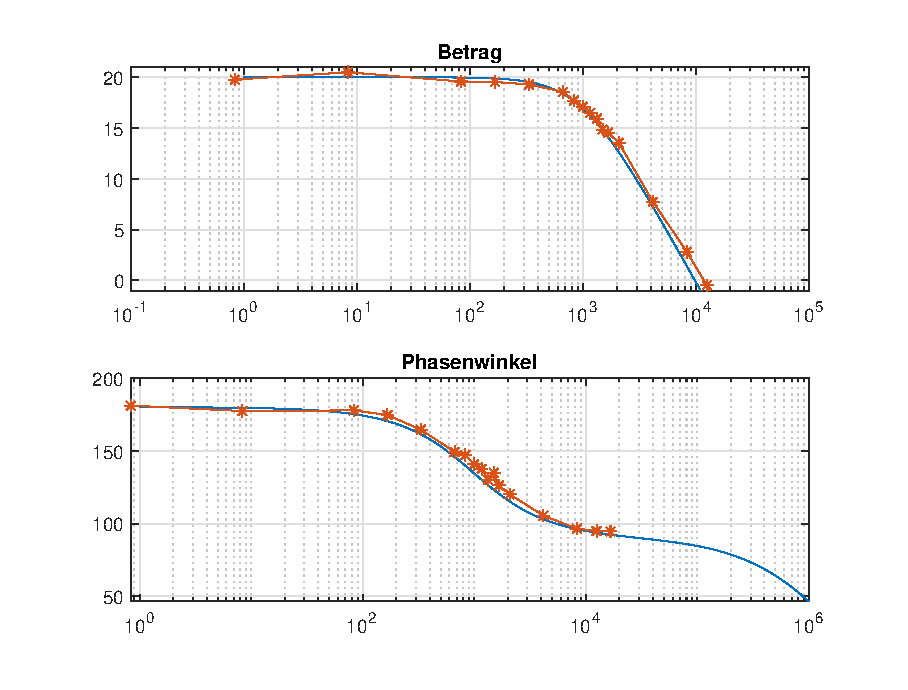
\includegraphics[width=\costumPicWidth]{Lab_2/Plots/TP_first_order.eps}
    \caption{Bodediagramm des Tiefpasses erster Ordnung}
    \label{fig:Bode_aktiver_Tiefpass}
\end{figure}
% Please add the following required packages to your document preamble:
% \usepackage[table,xcdraw]{xcolor}
% If you use beamer only pass "xcolor=table" option, i.e. \documentclass[xcolor=table]{beamer}
\begin{table}[]
\centering
\caption{Messergebnistabelle aktiver Tiefpass erster Ordnung}
\label{tab:TP_erg_tab}
\begin{tabular}{|l|l|l|l|}
\hline
\rowcolor[HTML]{C0C0C0} 
$f     $&$ U_{in} $&$ U_{out} $&$ Phase  $\\ \hline
$1\Hz     $&$ 95,85\mV  $&$ 932,66\mV  $&$ 181,04\degree $\\ \hline
$10\Hz    $&$ 88,37\mV  $&$ 935,18\mV  $&$ 177,33\degree $\\ \hline
$100\Hz   $&$ 97,74\mV  $&$ 931,16\mV  $&$ 177,77\degree $\\ \hline
$200\Hz   $&$ 98,49\mV  $&$ 933,17\mV  $&$ 174,57\degree $\\ \hline
$400\Hz   $&$ 98,12\mV  $&$ 904,52\mV  $&$ 164,48\degree $\\ \hline
$800\Hz   $&$ 97,49\mV  $&$ 826,13\mV  $&$ 149,25\degree $\\ \hline
$1\kHz   $&$ 101,26\mV $&$ 776,38\mV  $&$ 147,00\degree $\\ \hline
$1,2\kHz $&$ 101,88\mV $&$ 729,65\mV  $&$ 140,80\degree $\\ \hline
$1,4\kHz $&$ 102,51\mV $&$ 684,42\mV  $&$ 137,63\degree $\\ \hline
$1,6\kHz $&$ 102,26\mV $&$ 638,69\mV  $&$ 129,84\degree $\\ \hline
$1,8\kHz $&$ 108,29\mV $&$ 598,49\mV  $&$ 134,95\degree $\\ \hline
$2\kHz   $&$ 105,65\mV $&$ 563,82\mV  $&$ 126,22\degree $\\ \hline
$2,5\kHz $&$ 101,51\mV $&$ 482,91\mV  $&$ 120,11\degree $\\ \hline
$5\kHz   $&$ 112,19\mV $&$ 273,37\mV  $&$ 105,51\degree $\\ \hline
$10\kHz  $&$ 105,78\mV $&$ 146,23\mV  $&$ 96,53\degree  $\\ \hline
$15\kHz  $&$ 099,4\mV  $&$ 94,0\mV    $&$ 94,923\degree $\\ \hline
$20\kHz  $&$ 111,93\mV $&$ 80,40\mV   $&$ 94,685\degree $\\ \hline
\end{tabular}
\end{table}
In diesem Plot ist zu erkennen, dass die Grenzfrequenz bei der Simulation als auch bei den gemessenen Werten bei $f_g = 1kHz$ liegt. 

Der nächste Schritt war der Betrieb der Schaltung mit nicht-sinusförmigen Eingangsspanungen. Konkret wurde hier eine Rechteck und eine Dreieckspannung verwendet.

Um zu verstehen welche Messergebnisse hier zu erwarten sind, sollte an dieser Stelle ein Blick in die Übertragungsfunktion dieser Schaltung gewagt werden.

\begin{align}
    A = -\frac{R_2}{R_1}\frac{1}{1+sR_2 C}
\end{align}
Hier ist an dem Term $\frac{1}{s} $ zu erkennen, dass diese Schaltung integrierendes Verhalten zeigen muss. Durch Kenntnis der unbestimmten Integrale der Eingangsspannungen lassen sich nun Aussagen über die zu erwartenden Ausgangsspannungen treffen.
\subsubsection{Rechteckspannung}
\begin{align}
    \int{1 du} = u + c
\end{align}
Das heißt dass in diesem Fall eine linear ansteigend und abfallende Ausgangsspannung anliegen sollte.

Bei Rechteckspannung die sehr viel kleiner sind als die Grenzfrequenz ist eine Kondensatorladekurve zu sehen, was ebenfalls zu erwarten ist. 

\begin{figure}[H]
    \centering
    \includegraphics[width=\costumPicWidth]{Lab_2/Messungen/TP_first_order/scope_26.png}
    \caption{Rechteckspannung beim Tiefpass erster Ordnung $f < f_g$}
    \label{fig:Rechteck_Tiefpass_erster_Ordnung_small_f}
\end{figure}
\begin{figure}[H]
    \centering
    \includegraphics[width=\costumPicWidth]{Lab_2/Messungen/TP_first_order/scope_29.png}
    \caption{Rechteckspannung beim Tiefpass erster Ordnung $f > f_g$}
    \label{fig:Rechteck_Tiefpass_erster_Ordnung_big_f}
\end{figure}

\subsubsection{Dreieckspannung}
Auch in diesem Fall kann die Übertragungsfunktion zu Rate gezogen werden um eine Aussage über die erwartete Ausgangsspannung zu treffen. Bei dieser Eingangsspannung ist lediglich eine anderes unbestimmtes Integral zu lösen.

\begin{align}
    \int{u du} = \frac{1}{2} u^2 + c
\end{align}
Das heißt das nun eine parabelförmige Ausgangsspannung am Ausgang zu erwarten ist.

\begin{figure}[H]
    \centering
    \includegraphics[width=\costumPicWidth]{Lab_2/Messungen/TP_first_order/scope_30.png}
    \caption{Dreieckspannung beim Tiefpass erster Ordnung $f < f_g$}
    \label{fig:Dreieck_Tiefpass_erster_Ordnung_small_f}
\end{figure}
\begin{figure}[H]
    \centering
    \includegraphics[width=\costumPicWidth]{Lab_2/Messungen/TP_first_order/scope_34.png}
    \caption{Dreieckspannung beim Tiefpass erster Ordnung $f > f_g$}
    \label{fig:Dreieck_Tiefpass_erster_Ordnung_big_f}
\end{figure}
Wie zu erwarten ergab eine dreieckförmige Eingangsspannung eine Parabel als Ausgangsspannung
\subsection{Ausarbeitungen}
Gleich wie beim invertierenden Verstärker bildet sich am invertierenden Eingang ein virtueller Nullpunkt,
wodurch die Quelle nur durch den Widerstand $R_1$ belastet wird.

Die die Tiefpasswirkung, also die Trägheit, der Schaltung, verhindert schnelle Änderungen am Ausgang. Bei
niedrigen Frequenzen wären hohe Spannungen möglich, aber zusammen mit der niedrigen wird die Slew Rate
nicht überschritten. Bei gleicher Eingangsspannung aber einer höheren Frequenz wird das Signal stark
abgeschwächt, wodurch am Ausgang die Spannungsänderung pro Zeit auch klein bleibt. Diese Schaltung kann also
nicht bezüglich der Slew Rate übersteuert werden.

\begin{figure}[H]
    \centering
    \begin{circuitikz}[]
        \draw (0,0) node[op amp] (opamp) {$LM358$};
        \draw (opamp.up) --++(0,0.5) node[vcc]{$V_{CC}$};
        \draw (opamp.down) --++(0,-0.5) node[vee]{$V_{EE}$};
        \draw (opamp.+) to[short] ++(-0.5, 0) to[short] ++(0, -0.5) node[ground]{}; 
        
        \draw (opamp.-) to[R=$R_1$,-o] ++(-2,0) node[left]{$U_{in}$};
        \draw (opamp.-) to[short, *-] ++(0,2)
            to[R=$R_2$,*-*] ++(3,0)
            to[short,-*] ++(0,-2.5)
            to[short] (opamp.out);
        \draw (-1.2,2) to[R=$R_{Ref}$,*-o] ++(-2,0) node[left]{$U_{ref}$};
        \draw (opamp.-) to[short, *-] ++(0,3.5)
            to[C=$C$] ++(3,0)
            to[short] ++(0,-2);
        \draw (opamp.out) to[short, -o] (3,0) node[right]{$U_{out}$};
        \end{circuitikz}
    \caption{mögliche Schaltung zum Offsetabgleich}
    \label{fig:offsetabgleich_Tiefpass}
 \end{figure}

Die in Abbildung \ref{fig:offsetabgleich_Tiefpass} gezeigte Schaltung besitzt nun einen weiteren Eingang an welchem eine Referenzspannung angelegt werden kann. Damit kann ein Offsetabgleich durchgeführt werden, da sich dieser Eingang praktisch wie eine Additionsschaltung verhält und 

Laut Datenblatt müssen die möglichen Werte 2V unter der Versorgungsspannung liegen.

Die B-Endstufe des OPV steuert im Übergangsbereich zwischen positiver und negativer Ausgangsspannung
nicht exakt linear aus.
%%%%%%%%%%%%%%%%%%%%%%%%%%%%%%%%%%%%%%%%%%%%%%%%%%%%%%%%%%%%%%%%%%%%%%%%%%%%%%%%%%%%%%%%%%%%%%%%%%%%%%%%%%%%%%%%%%%%%%%%%%%%%%
\section{Hochpass erster Ordnung mit LM358}
\subsection{Aufgabenstellung}
Von dieser Schaltung ist messtechnisch die Grenzfrequenz zu ermitteln.

Es ist das Verhalten der Schaltung zu ermitteln wenn am Eingang Rechteck und Dreieckspannungen anliegen.

Das Bodediagramm der Schaltung ist zu ermitteln
\begin{figure}[H]
    \centering
    \begin{circuitikz}[]
        \draw (0,0) node[op amp] (opamp) {$LM358$};
        \draw (opamp.up) --++(0,0.5) node[vcc]{$V_{CC}$};
        \draw (opamp.down) --++(0,-0.5) node[vee]{$V_{EE}$};
        \draw (opamp.+) to[short] ++(-0.5, 0) to[short] ++(0, -0.5) node[ground]{}; 
        
        \draw (opamp.-) to[R=$R_1$] ++(-2,0) to[C=$C$,-o]++(-2,0) node[left]{$U_{in}$};
        \draw (opamp.-) to[short, *-] ++(0,2)
            to[R=$R_2$] ++(3,0)
            to[short,-*] ++(0,-2.5)
            to[short] (opamp.out);

        \draw (opamp.out) to[short, -o] (3,0) node[right]{$U_{out}$};
        \end{circuitikz}
    \caption{aktiver Hochpass erster Ordnung}
    \label{fig:Hochpass_LM358_Schaltung}
 \end{figure}

\subsection{Auslegung}
\begin{align}
    \nu = -\frac{R_2}{R_1} &= -10\\
    R_1 = 1k\Omega \Rightarrow R_2 &= 10k\Omega\\
    C = \frac{1}{2\pi f_g R_1} &= 15,9nF
\end{align}
\subsection{Messaufbau}
\begin{figure}[H]
    \centering
    \begin{circuitikz}[]
        \draw (0,0) node[op amp] (opamp) {$LM358$};
        \draw (opamp.up) --++(0,0.5) node[vcc]{$V_{CC}$};
        \draw (opamp.down) --++(0,-0.5) node[vee]{$V_{EE}$};
        \draw (opamp.+) to[short] ++(-0.5, 0) to[short] ++(0, -0.5) node[ground]{}; 
        
        \draw (opamp.-) to[R=$R_1$] ++(-2,0) to[C=$C$]++(-2,0) to[short] ++(-1,0)
            to[sV=CH1, color=white, name=S1,o-o] ++(0,-2) node[ground] {}
            to[short,o-] ++(-2,0)
            to[sV] ++(0,2)
            to[short,-o] ++(2,0);
            
        \draw (opamp.-) to[short, *-] ++(0,2)
            to[R=$R_2$] ++(3,0)
            to[short,-*] ++(0,-2.5)
            to[short] (opamp.out);

        \draw (opamp.out) to[short, -o] (3,0) to[sV=CH2, color=white, name=S2,o-o] ++(0,-2) node[ground]{};
        
        \myscope{S1}{0}
        \myscope{S2}{0}
        \end{circuitikz}
    \caption{aktiver Hochpass erster Ordnung}
    \label{fig:Hochpass_LM358_Messaufbau}
 \end{figure}

\subsection{Messergebnisse}
\begin{figure}[H]
    \centering
    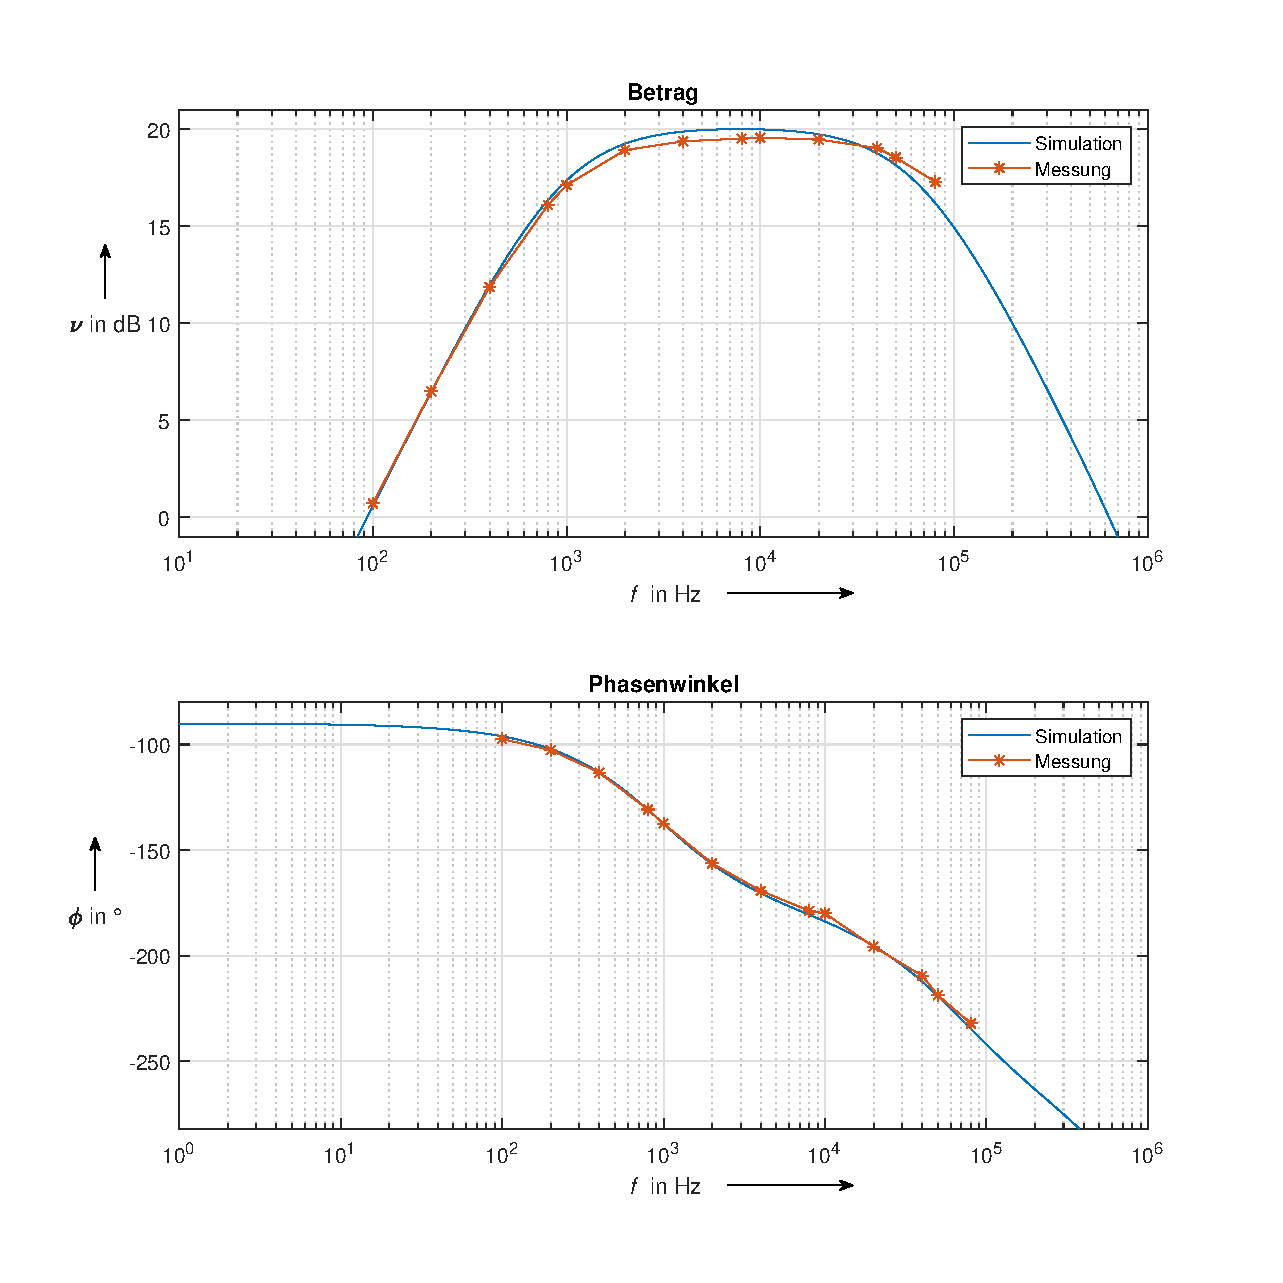
\includegraphics[width=\costumPicWidth]{Lab_2/Plots/HP_first_order.eps}
    \caption{Bodediagramm des Hochpass erster Ordnung}
    \label{fig:Bode_HP_first_order}
\end{figure}
% Please add the following required packages to your document preamble:
% \usepackage[table,xcdraw]{xcolor}
% If you use beamer only pass "xcolor=table" option, i.e. \documentclass[xcolor=table]{beamer}
\begin{table}[H]
\centering
\caption{Messergebnistabelle aktiver Hochpass erster Ordnung}
\label{tab:HP_erg_tab}
\begin{tabular}{|r|r|r|r|}
\hline
\rowcolor[HTML]{C0C0C0} 
$f\text{ in }\Hz$       & $U_{in}\text{ in }\mV$    & $U_{out}\text{ in }\mV$   & $\phi\text{ in }\degree$        \\ \hline
$100  $&$ 100,7 $&$ 109,4  $&$ 97,43  $\\ \hline
$200  $&$ 100,5 $&$ 212,3  $&$ 102,63 $\\ \hline
$400  $&$ 99,6  $&$ 391,0  $&$ 113,28 $\\ \hline
$800  $&$ 98,9  $&$ 631,2  $&$ 130,78 $\\ \hline
$1\Kilo  $&$ 98,3  $&$ 706,5  $&$ 137,47 $\\ \hline
$2\Kilo  $&$ 97,8  $&$ 865    $&$ 156,33 $\\ \hline
$4\Kilo  $&$ 99,0  $&$ 923    $&$ 169,31 $\\ \hline
$8\Kilo  $&$ 99,1  $&$ 939    $&$ 178,75 $\\ \hline
$10\Kilo $&$ 98,7  $&$ 940    $&$ 180,00 $\\ \hline
$20\Kilo $&$ 98,5  $&$ 928    $&$ 195,73 $\\ \hline
$40\Kilo $&$ 98,6  $&$ 883    $&$ 209,57 $\\ \hline
$50\Kilo $&$ 99,7  $&$ 844    $&$ 218,74 $\\ \hline
$80\Kilo $&$ 100,9 $&$ 739,00 $&$ 232,1 $\\ \hline
\end{tabular}
\end{table}
\begin{figure}[H]
    \centering
    \includegraphics[width=\costumPicWidth]{Lab_2/Messungen/HP_first_order/scope_70.png}
    \caption{Messtechnische Erfassung der Grenzfrequenz}
    \label{fig:HP_FO_fg}
\end{figure}
\subsubsection{Rechteckspannung}
Auch hier ist wieder zu sehen, dass sich die Ausgangsspannung wie mathemtatisch zu erwarten verhält.
\begin{align}
    \frac{dx}{dt}1=\frac{1}{x}\\
    \frac{dx}{dt}x = 1
\end{align}
\begin{figure}[H]
    \centering
    \includegraphics[width=\costumPicWidth]{Lab_2/Messungen/HP_first_order/scope_66.png}
    \caption{Bodediagramm des Hochpass erster Ordnung}
    \label{fig:Bode_HP_first_order}
\end{figure}
\begin{figure}[H]
    \centering
    \includegraphics[width=\costumPicWidth]{Lab_2/Messungen/HP_first_order/scope_53.png}
    \caption{Bodediagramm des Hochpass erster Ordnung}
    \label{fig:Bode_HP_first_order}
\end{figure}

\subsubsection{Dreieckspannung}
\begin{figure}[H]
    \centering
    \includegraphics[width=\costumPicWidth]{Lab_2/Messungen/HP_first_order/scope_5.png}
    \caption{Dreieckspannung $f<f_g$}
    \label{fig:HP_FO_Dreieck_kleiner}
\end{figure}
\begin{figure}[H]
    \centering
    \includegraphics[width=\costumPicWidth]{Lab_2/Messungen/HP_first_order/scope_2.png}
    \caption{Dreieckspannung $f>f_g$}
    \label{fig:HP_FO_Dreieck}
\end{figure}

\subsection{Ausarbeitungen}
Da das Kleinsignalverhalten immer für sehr hohe Frequenzen bestimmt wird (also alle Kapazitäten leitend), beträgt der Eingangswiderstand dieser Schaltung den Wert $R_1$. Im Gleichspannungsfall würde dieser unendlich hoch sein, da die Kapazität in diesem Fall sperrend wirkt.

Diese Schaltung kann hinsichtlich der Slew Rate auf alle Fälle übersteuern, da die Verstärkung vor allem hohe Frequenzen betrifft.

\chapter{Operationsverstärker - Anwendungen}
\section{Präzisionsgleichrichter mit LM358}
\subsection{Aufgabenstellung}
Die Schaltung aus \autoref{fig:Gleichrichter_Schaltung} ist auf einem Steckbrett aufzubauen, dabei ist das Verhalten mit und ohne dem Kondensator C zu dokumentieren. Außerdem ist der Frequenzbereich zu bestimmen in welchem der Fehler der Schaltung bei unter 1\% bleibt.
\begin{figure}[H]
    \centering
    \begin{circuitikz}[]
        \draw (0,0) node[op amp] (opamp) {$LM358$};
        \draw (opamp.up) --++(0,0.5) node[vcc]{$V_{CC}$};
        \draw (opamp.down) --++(0,-0.5) node[vee]{$V_{EE}$};
        \draw (opamp.+) to[short] ++(-0.5, 0) to[short] ++(0, -0.5) node[ground]{}; 
        
        \draw (opamp.-) to[R=$R$,-o] ++(-3,0) node[left]{$U_{in}$};
        \draw (opamp.-) to[short, *-] ++(0,4) 
            to[R=$R$,-*] ++(3,0) 
            to[D, -*] ++(0,-2) 
            to[D,-*]++(-3,0);
        \draw (opamp.out) to[short] ++(0.616161616161616,0) to[short] ++(0,3);
        \draw (1.5,4.5) to[short] ++(2,0)
            to[sR=$R$, name=sR] ++(0,-3)
            to[short] ++(0,-5)
            to[R=$R$] ++(-7.25,0)
            to[short,-*] ++(0,4);
            
        \draw (sR.label) to[short] ++(0,0.75)
            to[short,-*] ++(0.35,0);
        
        \draw (7,1) node[op amp] (opamp2) {$LM358$};
        \draw (opamp2.up) --++(0,0.5) node[vcc]{$V_{CC}$};
        \draw (opamp2.down) --++(0,-0.5) node[vee]{$V_{EE}$};
        \draw (opamp2.+) to[short] ++(-0.5, 0) to[short] ++(0, -0.5) node[ground]{};         
        
        \draw (opamp2.-) to[short,-*] ++(-2.3,0);
        
        \draw (opamp2.-) to[short, *-] ++(0,2)
            to[R=$R$,*-*] ++(3,0)
            to[short,-*] ++(0,-2.5)
            to[short] (opamp2.out);
        \draw (opamp2.-) to[short, *-] ++(0,3.5)
            to[C=$C$] ++(3,0)
            to[short] ++(0,-2);
        \draw (opamp2.out) to[short, -o] ++(1,0) node[right]{$U_{out}$};
        
        \end{circuitikz}
    \caption{Präzisionsgleichrichter mit LM358}
    \label{fig:Gleichrichter_Schaltung}
 \end{figure}

\subsection{Messaufbau}
Die Schaltung wurde mit dem Signalgenerator betrieben und mit $V_{CC} = -V_{EE} = 15V$ versorgt. Der Ausgang der Schaltung wurde mit dem Oszilloskop erfasst. Bei der Messung des Gleichrichtwertes wurde zusätzlich mit dem Tischmultimeter gemessen.
\subsection{Auslegung der Schaltung}
Alle verwendeten Widerstände wurden mit dem Nominalwert $R=10k\Omega$ ausgelegt. Das hat einerseits den Vorteil, dass die Quelle nur eine sehr geringe Last erfährt und andererseits hatten wir einen $R_{Trim} = 10k\Omega$ Trimmer zur Verfügung. Dieser wurde eingebaut um Bauteiltoleranzen kompensieren zu können und dafür zu sorgen, dass beide Halbwellen des gleichgerichteten Sinus gleich groß sind.

Für die beiden Dioden wurde das Modell 1N4148 verwendet.
\subsection{Interpretation der Messergebnisse}
Wie in Abbildung \ref{fig:sim_Gleichrichter} zu sehen ist, ist für den Aufbau ohne dem Glättungskondesator C ein gleichgerichter Sinus zu erwarten. Für den Aufbau mit C ist eine schwach pulsierende Gleichspannung zu erwarten die dem Gleichrichtwert des Sinus entspricht.
\subsubsection{Gleichrichtwert einer Sinusspannung}
Für die Herleitung dieses Wertes ist die Phasenverschiebung des Eingangssignals irrelevant. Sie wurde deswegen mit $\phi_x = 0$ angenommen. 
\begin{align}
    u(t)_{Signal} =  \hat{u} \cdot \sin(\omega t) \\   
    u_{glr} = \int_{0}{|u(t)_{Signal}|} \\
\end{align}
Da im Falle des gleichgerichteten Sinus das Signal bereits bei $\frac{T}{2}$ periodisch ist gilt:
\begin{align}
x_{glr} = \frac{1}{\frac{T}{2}}\int _{0} ^{\frac{T}{2}} |\hat{x} \cdot \sin{(\omega t)}|dt\\
x_{glr} = \frac{2\hat{x}}{T} \bigl\lbrack -\frac{1}{\omega}\cos{(\omega t)} \bigr\rbrack ^{\frac{T}{2}} _{t=0} \\
x_{glr} = \frac{2}{\pi} \hat{x} = 0,6366\cdot \hat{x}
\end{align}

Das heißt in diesem Fall ist ein Wert der tiefpassgefilterten Spannung von $U_{gr} =\frac{2}{\pi}\cdot U_{pp}$ zu erwarten. Nun wurde die Frequenz erhöht bis eine Abweichung von 1\% von diesem Wert gemessen wurde. Dieser Umstand trat bei einer Frequenz von $f=6,5\kHz$

\begin{figure}[H]
    \centering
    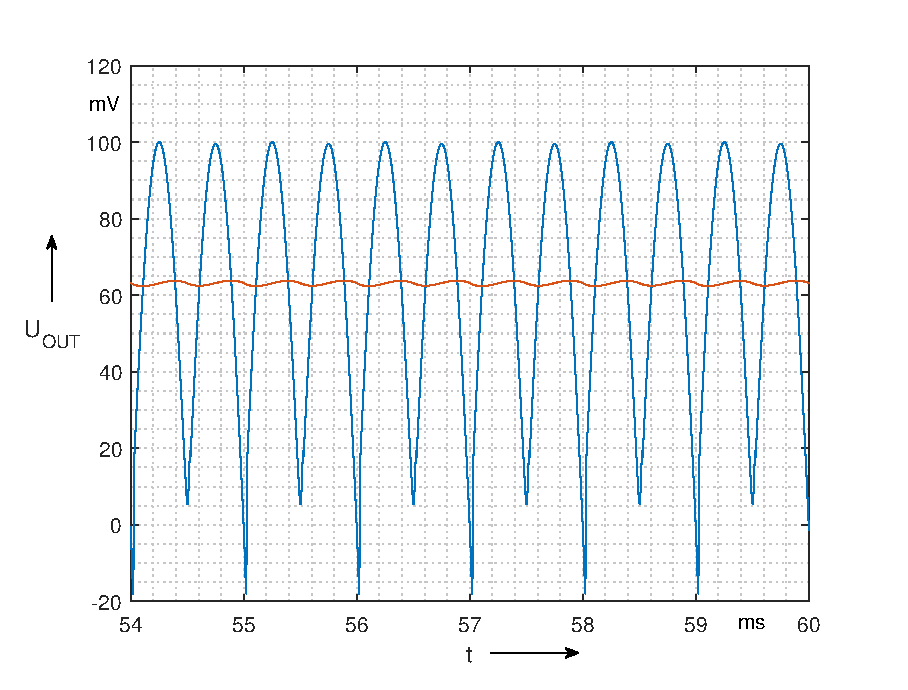
\includegraphics[width=\costumPicWidth]{Lab_3/Plots/Gleichrichter.eps}
    \caption{Simulationsergebnisse des Präzisionsgleichrichters}
    \label{fig:sim_Gleichrichter}
\end{figure}

\begin{figure}[H]
    \centering
    \includegraphics[width=\costumPicWidth]{Lab_3/Messungen/scope_1.png}
    \caption{Gleichrichter ohne C}
    \label{fig:res_gleichrichter_ohne_C}
\end{figure}
\begin{figure}[H]
    \centering
    \includegraphics[width=\costumPicWidth]{Lab_3/Messungen/scope_2.png}
    \caption{Gleichrichter mit C}
    \label{fig:res_gleichrichter_mit_C}
\end{figure}
\subsection{Ausarbeitungen}
Ja, für diese Schaltung ist eine Art Offsetabgleich erforderlich. In unserem Fall wurde dies durch den einstellbaren Widerstand $^R/_2$ erreicht worden.

Hier handelt es sich um den arithmetischen Mittelwert. Dieser entspricht dem Gleichrichtwert eines Eingangssignals.
%%%%%%%%%%%%%%%%%%%%%%%%%%%%%%%%%%%%%%%%%%%%%%%%%%%%%%%%%%%%%%%%%%%%%%%%%%%%%%%%%%%%%%%%%%%%%%%

\section{Single Supply Mikrofonverstärker mit LM358 und AD823}
\subsection{Aufgabenstellung}
Die Schaltung aus Abbildung \ref{fig:Mikrofon_Schaltung} soll bei einer Frequenz von $f=30Hz$ eine Verstärkung von $\nu = 40dB$ haben. 
Danach soll die Schaltung auf dem Steckbrett aufgebaut werden und ein Frequenzgang erfasst werden.

Auf einen Versuch mit Mikrofon und Lautsprecher wurde heuer wegen geringerer Laborzeit verzichtet. 

Nach Aufnahme des Amplitudengangs der Schaltung mit dem LM358 wird der Operationsverstärker mit dem pinkompatiblen AD823 ersetzt. Nun wird der Amplitudengang erneut aufgenommen. Diese beiden Amplitudengänge sind zu vergleichen. 
\begin{figure}[H]
    \centering
    \begin{circuitikz}[]
        \draw (0,0) node[op amp,yscale=-1] (opamp) {\scalebox{1}[-1]{$LM358$}};
        \draw (opamp.down) --++(0,0.5) node[vcc]{$V_{CC}$};
        \draw (opamp.up) --++(0,-0.5) node[vee]{$V_{EE}$};

        \draw (opamp.+) to[short] ++(-2,0) to[C=$C_1$,-o] ++(-2,0) node[left]{$U_{in}$};
        \draw (-3,0.5) to[R=$R_5$,*-] ++(0,2) node[vcc]{$V_{CC}$};
        \draw (-3,0.5) to[R=$R_4$,*-] ++(0,-2) node[ground]{};
        
        \draw (opamp.-) to[short] ++(-0.5,0)
            to[short] ++(0,-3)
            to[R=$R_2$] ++(0,-1.5)
            to[C=$C_3$] ++(0,-1.5) node[ground]{};
        \draw (opamp.out) to[short] ++(2,0)
            to[C=$C_2$,-o] ++(1.5,0) node[right]{$U_{out}$};
        \draw (3,0) to[R=$R_3$,*-] ++(0,-2) node[ground]{};
        \draw (2,0) to[short, *-] ++(0,-2.5)
            to[R=$R_1$,-*] ++(-3.7,0);
        \end{circuitikz}
    \caption{Mikrofonverstärker mit LM358 und AD823}
    \label{fig:Mikrofon_Schaltung}
 \end{figure}

\subsection{Messaufbau}
\subsection{Auslegung der Schaltung}
Die Schaltung soll bei $f=30Hz$ bereits eine Verstärkung von $\nu = -100$ aufweisen. Deswegen wurde die Grenzfrequenz der Schaltung mit $f_g=5Hz$ festgelegt. 
Dazu wurden ein paar der Widerstandswerte im Vorhinein angenommen. Mit dem damit resultierenden Tiefpass kann die Kapazität $C_1$ ausgelegt werden.
\begin{align}
    R_4=R_5 &= 100k\Omega \\
    R_{in} = \frac{R_4\cdot R_5}{R_4+ R_5} &= 50k\Omega \\
    C_1=\frac{1}{2\pi f_g R_{in}} = \frac{1}{2\cdot \pi \cdot 5\cdot50\cdot 10^3} &= 636.61nF \approx 2\cdot 330nF = 660nF
\end{align}
Durch die gegebene Verstärkung kann nun der Spannungsteiler $R_1$ und $R_2$ und die Kapazität $C_3$ ausgelegt werden. Die beiden hier verwendeten Widerstände sollten zwar ausreichend groß, jedoch nicht zu groß gewählt werden, da in diesem Bereich der Schaltung parasitäre Kapazitäten sehr leicht zu einem Tiefpassverhalten führen können. Besonders durch den Aufbau auf einem Steckbrett ist diese Schaltung anfällig dafür. 
\begin{align}
    R_1 &= 100k\Omega\\
    \nu = -100 &= -\frac{R_1}{R_2} \\
    R_2 = \frac{R_1}{\nu} &= 1k\Omega\\
    C_3=\frac{1}{2\pi f_g R_2} = \frac{1}{2\cdot \pi \cdot 5\cdot1\cdot 10^3} &= 31,813\mu F \approx 32\mu F
\end{align}
Da die Kapazität $C_2$ lediglich für eine kapazitive Kopplung der Schaltung sorgen soll, wurde ihr Wert willkürlich auf $C_2=100nF$ festgelegt. 

\begin{table}[H]
\centering
\caption{Bauteilwerte Mikrofonverstärker}
\label{tab:Bauteile_Mikrofonv}
\begin{tabular}{|l|r|r|}
\hline
\rowcolor[HTML]{C0C0C0} 
Bauteilname & \multicolumn{1}{l|}{\cellcolor[HTML]{C0C0C0}gewählter Wert} & \multicolumn{1}{l|}{\cellcolor[HTML]{C0C0C0}gemessener Wert} \\ \hline
$R_1$       & $100k\Omega$                                                & $99,491k\Omega$                                              \\ \hline
$R_2$       & $1k\Omega$                                                  & $1,0007k\Omega$                                              \\ \hline
$R_3$       & $100k\Omega$                                                & $98,098k\Omega$                                              \\ \hline
$R_4$       & $100k\Omega$                                                & $99,520k\Omega$                                              \\ \hline
$R_5$       & $100k\Omega$                                                & $98,422k\Omega$                                              \\ \hline
$C_1$       & $660nF$                                                     & $644nF$                                                      \\ \hline
$C_2$       & $100nF$                                                     & $98,5nF$                                                     \\ \hline
$C_3$       & $32\mu F$                                                   & $38,0\mu F$                                                  \\ \hline
\end{tabular}
\end{table}

\subsection{Messergebnisse}
\begin{figure}[H]
    \centering
    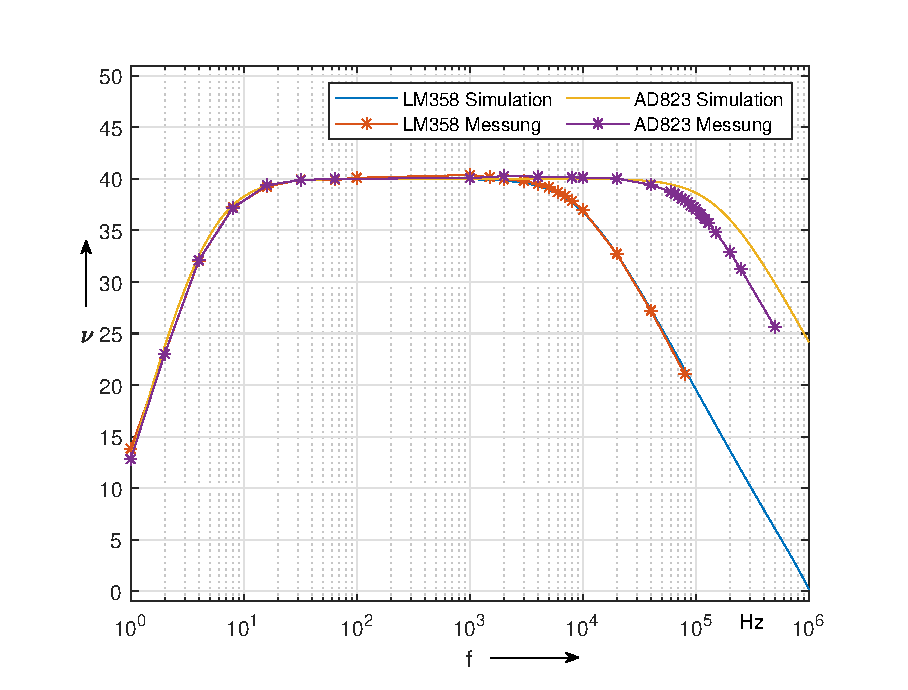
\includegraphics[width=\costumPicWidth]{Lab_3/Plots/Mikrofonverstaerker.eps}
    \caption{Vergleich der Amplitudengänge beim Mikrofonverstärker}
    \label{fig:Amplitudengang_Mikverstaerker}
\end{figure}
% Please add the following required packages to your document preamble:
% \usepackage[table,xcdraw]{xcolor}
% If you use beamer only pass "xcolor=table" option, i.e. \documentclass[xcolor=table]{beamer}
\begin{table}[]
\centering
\caption{Messergebnisstabelle Mikrofonverstärker}
\label{tab:Mikrofon_erg_tab}
\begin{tabular}{l||l|l||l|l|}
\cline{2-5}
                                                & \multicolumn{2}{l|}{AD523} & \multicolumn{2}{l|}{LM358} \\ \hline
\rowcolor[HTML]{C0C0C0} 
\multicolumn{1}{|l|}{\cellcolor[HTML]{C0C0C0}$f$} &$ U_{in}       $&$ U_{out}     $&$ U_{in}       $&$ U_{out}  $\\ \hline
\multicolumn{1}{|l|}{$1\Hz$}                         &$ 51,457\mV    $&$ 221,11\mV   $&$ 51,457\mV   $&$ 248,24\mV    $\\ \hline
\multicolumn{1}{|l|}{$2\Hz$}                         &$ 51,960\mV    $&$ 713,07\mV   $&$ 51,859\mV   $&$ 710,55\mV    $\\ \hline
\multicolumn{1}{|l|}{$4\Hz$}                         &$ 51,357\mV    $&$ 1,9812\Hz      $&$ 51,558\mV   $&$ 1,9799\Hz       $\\ \hline
\multicolumn{1}{|l|}{$8\Hz$}                         &$ 51,558\mV    $&$ 3,5377\Hz      $&$ 51,859\mV   $&$ 3,5879\Hz       $\\ \hline
\multicolumn{1}{|l|}{$16\Hz$}                        &$ 51,055\mV    $&$ 4,5176\Hz      $&$ 51,156\mV   $&$ 4,4526\Hz       $\\ \hline
\multicolumn{1}{|l|}{$32\Hz$}                        &$ 51,357\mV    $&$ 4,8015\Hz      $&$ 51,457\mV   $&$ 4,8291\Hz       $\\ \hline
\multicolumn{1}{|l|}{$64\Hz$}                        &$ 51,558\mV    $&$ 4,8894\Hz      $&$ 51,960\mV   $&$ 4,8844\Hz       $\\ \hline
\multicolumn{1}{|l|}{$100\Hz$}                       &$              $&$             $&$ 51,558\mV   $&$ 4,9422\Hz       $\\ \hline
\multicolumn{1}{|l|}{$1\kHz$}                       &$ 51,960\mV    $&$ 4,9598\Hz      $&$ 049,6\mV    $&$ 4,905\Hz        $\\ \hline
\multicolumn{1}{|l|}{$1,5\kHz$}                     &$              $&$             $&$ 050,5\mV    $&$ 4,872\Hz        $\\ \hline
\multicolumn{1}{|l|}{$2\kHz$}                       &$ 050,4\mV     $&$ 4,917\Hz       $&$ 51,10\mV    $&$ 4,821\Hz        $\\ \hline
\multicolumn{1}{|l|}{$3\kHz$}                       &$              $&$             $&$ 050,5\mV    $&$ 4,681\Hz        $\\ \hline
\multicolumn{1}{|l|}{$4\kHz$}                       &$ 050,6\mV     $&$ 4,915\Hz       $&$ 050,9\mV    $&$ 4,560\Hz        $\\ \hline
\multicolumn{1}{|l|}{$5\kHz$}                       &$              $&$             $&$ 050,9\mV    $&$ 4,384\Hz        $\\ \hline
\multicolumn{1}{|l|}{$6\kHz$}                       &$              $&$             $&$ 051,3\mV    $&$ 4,196\Hz        $\\ \hline
\multicolumn{1}{|l|}{$7\kHz$}                       &$              $&$             $&$ 051,0\mV    $&$ 4,000\Hz        $\\ \hline
\multicolumn{1}{|l|}{$8\kHz$}                       &$ 050,5\mV     $&$ 4,864\Hz       $&$ 051,4\mV    $&$ 3,812\Hz        $\\ \hline
\multicolumn{1}{|l|}{$10\kHz$}                      &$ 050,6\mV     $&$ 4,864\Hz       $&$ 051,0\mV    $&$ 3,427\Hz        $\\ \hline
\multicolumn{1}{|l|}{$20\kHz$}                      &$ 050,8\mV     $&$ 4,824\Hz       $&$ 051,3\mV    $&$ 2,126\Hz        $\\ \hline
\multicolumn{1}{|l|}{$40\kHz$}                      &$ 051,2\mV     $&$ 4,545\Hz       $&$ 051,6\mV    $&$ 1,141\Hz        $\\ \hline
\multicolumn{1}{|l|}{$60\kHz$}                      &$ 051,6\mV     $&$ 4,239\Hz       $&$             $&$              $\\ \hline
\multicolumn{1}{|l|}{$65\kHz$}                      &$ 051,4\mV     $&$ 4,131\Hz       $&$             $&$              $\\ \hline
\multicolumn{1}{|l|}{$70\kHz$}                      &$ 051,5\mV     $&$ 4,043\Hz       $&$             $&$              $\\ \hline
\multicolumn{1}{|l|}{$75\kHz$}                      &$ 051,7\mV     $&$ 3,940\Hz       $&$             $&$              $\\ \hline
\multicolumn{1}{|l|}{$80\kHz$}                      &$ 051,4\mV     $&$ 3,839\Hz       $&$ 052,0\mV    $&$ 570,9\mV     $\\ \hline
\multicolumn{1}{|l|}{$85\kHz$}                      &$ 051,3\mV     $&$ 3,751\Hz       $&$             $&$              $\\ \hline
\multicolumn{1}{|l|}{$90\kHz$}                      &$ 051,8\mV     $&$ 3,658\Hz       $&$             $&$              $\\ \hline
\multicolumn{1}{|l|}{$95\kHz$}                      &$ 051,4\mV     $&$ 3,565\Hz       $&$             $&$              $\\ \hline
\multicolumn{1}{|l|}{$100\kHz$}                     &$ 051,4\mV     $&$ 3,480\Hz       $&$             $&$              $\\ \hline
\multicolumn{1}{|l|}{$110\kHz$}                     &$ 051,5\mV     $&$ 3,307\Hz       $&$             $&$              $\\ \hline
\multicolumn{1}{|l|}{$120\kHz$}                     &$ 051,7\mV     $&$ 3,151\Hz       $&$             $&$              $\\ \hline
\multicolumn{1}{|l|}{$130\kHz$}                     &$ 051,6\mV     $&$ 3,003\Hz       $&$             $&$              $\\ \hline
\multicolumn{1}{|l|}{$150\kHz$}                     &$ 052,0\mV     $&$ 2,729\Hz       $&$             $&$              $\\ \hline
\multicolumn{1}{|l|}{$200\kHz$}                     &$ 052,3\mV     $&$ 2,209\Hz       $&$             $&$              $\\ \hline
\multicolumn{1}{|l|}{$250\kHz$}                     &$ 052,3\mV     $&$ 1,829\Hz       $&$             $&$              $\\ \hline
\multicolumn{1}{|l|}{$500\kHz$}                     &$ 052,3\mV     $&$ 965\mV      $&$             $&$              $\\ \hline
\end{tabular}
\end{table}
\subsection{Interpretation der Messergebnisse} 
Wie in Abbildung \ref{fig:Amplitudengang_Mikverstaerker} zu erkennen ist verhalten sich die real gemessenen Werte, sowie die Schaltungen mit beiden Operationsverstärkern nahezu ident. Die untere Grenzfrequenz liegt bei ungefähr $f_g=8Hz$, das führt dazu, dass bei 30Hz schon nahezu eine Verstärkung von $\nu = 40dB$ erreicht ist.

Bei der oberen Grenzfrequenz ist jedoch nun gut zu erkennen, dass der LM358 das Band bereits sehr viel früher begrenzt, als der AD823. Hier stimmen auch die simulierten Werte mit den gemessenen sehr gut überein. Das liegt vorrangig daran, dass parasitäre Kapauzäten bei solch geringen Frequenzen sehr wenig Einfluss auf die Schaltung haben.

Beim Vergleich der Simulation und der Messung der Schaltung mit dem AD823 ist eine deutlich höhere obere Grenzfrequenz auszumachen. Diese ist bei der gemessenen Schaltung etwas früher, was aber vermutlich an parasitären Kapazitäten im Steckbrett liegt. Dies musste ich während der Laboreinheit erfahren, da der erste Aufbau mit deutlich größeren Widerstandswerten aufgebaut wurde, um die Kapazität $C_3$ möglichst klein zu halten. Dabei erzeugt die Kapazität des Steckbrettes bereits bei $f_g=10^4Hz$ eine obere Grenzfrequenz. 

Für Audioanwendungen ist der AD823 gut geeignet, da der menschliche Hörbereich ungefähr von 16 - 20.000 Hz angegeben wird und die obere Grenzfrequenz bei diesem Verstärker jenseits der 50kHz ist.  Desweiteren beträgt die Samplerate bei MP3 ohnehin nur 44,2kHz, wobei nach dem Abtasttheorem nach Shannon - Nyquist Töne bis maximal 22,1 kHz wiederhergestellt werden können. Der LM358 ist jedenfalls nicht geeignet. Er zeigt bereits bei deutlich zu niedrigen Frequenzen ein Tiefpassverhalten und würde die Qualität des aufgenommenen Signals stark verringern. 
\subsection{Ausarbeitungen}

\section{Sallen-Key Tiefpassfilter}
\subsection{Aufgabenstellung}
Die Schaltung aus Abbildung \ref{fig:Sallen_key} ist auf eine $f_g=30Hz$ und auf eine Verstärkung von $\nu = +10$ auszulegen. Der Filter soll eine Butterworth Charakteristik aufweisen und mit dem Operationsverstärker AD823 auf dem Steckbrett aufgebaut werden.

Von dieser Schaltung ist während der Laboreinheit kein Bodediagramm aufzunehmen. 
\begin{figure}[H]
    \centering
    \begin{circuitikz}[]
        \draw (0,0) node[op amp,yscale=-1] (opamp) {\scalebox{1}[-1]{$AD823$}};
        \draw (opamp.down) --++(0,0.5) node[vcc]{$V_{CC}$};
        \draw (opamp.up) --++(0,-0.5) node[vee]{$V_{EE}$};
        
        \draw (opamp.+) to[short, -*] ++(-2,0)
            to[C=$C_2$] ++(0,-2) node[ground]{};
        \draw (opamp.+) to[short, -*] ++(-2,0)
            to[R=$R_2$] ++(-2,0)
            to[R=$R_1$,-o] ++(-2,0) node[left]{$U_{in}$};
        \draw (-5.25,0.5) to[short,*-] ++(0,2)
            to[C=$C_1$] ++(7.445,0)
            to[short] ++(0,-2.5)
            to[short] (opamp.out);
        \draw (opamp.out) to[short,-*] ++(1,0)
            to[R=$R_4$,-*] ++(0,-3)
            to[R=$R_3$] ++(0,-2) node[ground]{};
        \draw (2.2,-3) to[short] ++(-4,0)
            to[short] ++(0,2.5)
            to[short] (opamp.-);
        \draw (opamp.out) to[short,-o] ++(2,0) node[right] {$U_{out}$};
        \end{circuitikz}
    \caption{Sallen-key, Aktiver Tiefpass}
    \label{fig:Sallen_key}
 \end{figure}


\subsection{Auslegung}
Zur Auslegung dieser Schaltung ist die Übertragungsfunktion \cite[212]{10.5555/3158302} sehr hilfreich.

\begin{align}
    A(s) = \frac{A_0}{1+a_1s + b_1s^2}&=\frac{A_0}{1+\omega_c[C_1(R_1+R_2) + (1-A_0)R_1C_2]s + {\omega_C}^2R_1R_2C_1C_2s^2} \\
    \rm mit \it A_0 &= 1+ \frac{R_4}{R_3} 
\end{align}
Da dieser Filter eine Butterworth Charakteristik aufweisen soll, gilt für $a_1$ und $b_1$:

\begin{align}
    a_1 &= \sqrt{2} \\
    b_1 &= 1
\end{align}

Damit gilt: 
\begin{align}
    a_1 = \sqrt{2} &= \omega_c[C_1(R_1+R_2) + (1-A_0)R_1C_2] \label{eq:a1}\\
    b_1 = 1 &= {\omega_C}^2R_1R_2C_1C_2 \label{eq:b1}
\end{align}

Da im Labor wesentlich weniger verschiedene Kapazitätswerte als Widerstandswerte verfügbar sind, wurde mit der Wahl der Kapazitäten $C_1$ und $C_2$ begonnen. Im Falle der Auslegung einer Schaltung für den realen Einsatz sollte bei der Wahl dieser Kapazitäten auf geringe Toleranzen vom Absolutwert und bei Temperaturdrift wert gelegt werden. Im Labor waren ohnehin nur Kapazitäten mit $\pm10\%$ verfügbar. 

\begin{align}
    C_1 &= 100nF \\
    C_2 &= 330nF
\end{align}

Nach Umformen der Gleichungen \ref{eq:a1} und \ref{eq:b1} ergaben sich folgende Widerstandswerte:

\begin{align}
    R_1 &= 4,28k\Omega \\
    R_2 &= 198,4 k\Omega
\end{align}

\lstinputlisting[language = Matlab, caption=matlab Skript zur Auslegung des aktiven Filter]{Lab_3/auslegung_Sallen_key.m}

\subsection{Simulationsergebnisse}
\begin{figure}[h]
    \centering
    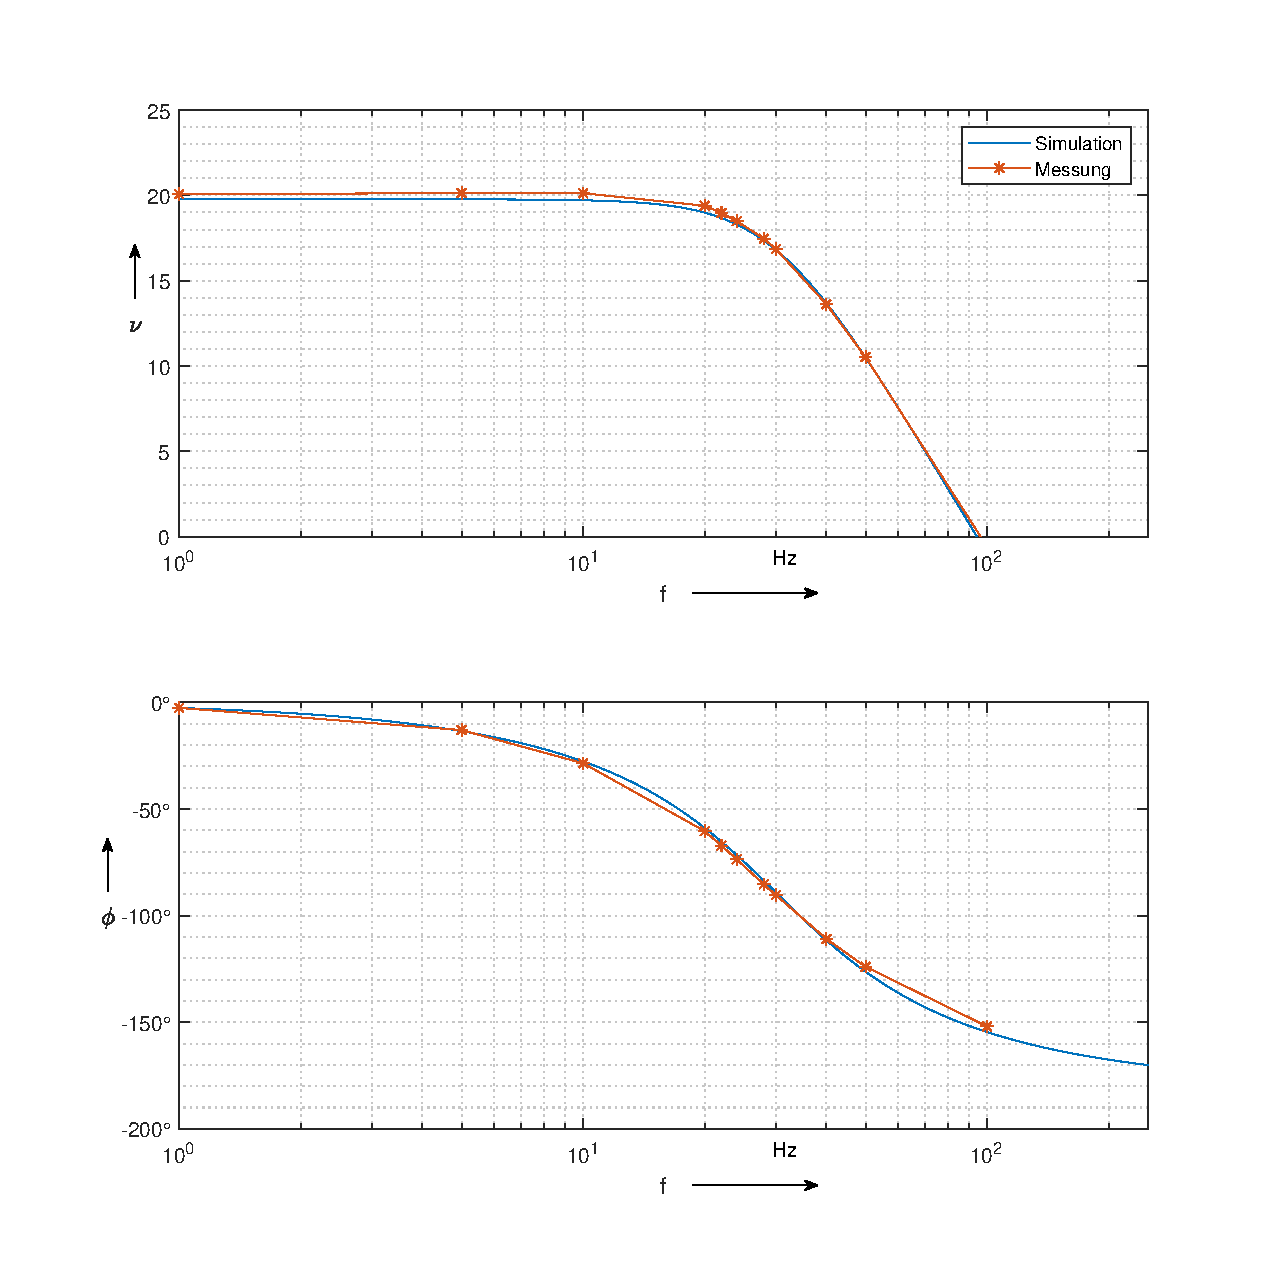
\includegraphics[width = \costumPicWidth]{Lab_3/Plots/sallen_key.eps}
    \caption{Bodediagramm aktiver Tiefpass 2. Ordnung}
    \label{fig:my_label}
\end{figure}

% Please add the following required packages to your document preamble:
% \usepackage[table,xcdraw]{xcolor}
% If you use beamer only pass "xcolor=table" option, i.e. \documentclass[xcolor=table]{beamer}
\begin{table}[H]
\centering
\caption{Messergebnistabelle Sallen-Key Filter}
\label{tab:sallen_key_erg_table}
\begin{tabular}{|r|r|r|r|}
\hline
\rowcolor[HTML]{C0C0C0} 
$f\text{ in }\Hz   $&$ U_{in}\text{ in }\V       $&$ U_{out}\text{ in }\V     $&$ \phi\text{ in }\degree   $\\ \hline
$1   $&$ 989,95\text{m} $&$ 9,9849   $&$ -2,633  $\\ \hline
$5   $&$ 990,95\text{m} $&$ 10,060   $&$ -13,05  $\\ \hline
$10  $&$ 1,0030    $&$ 10,176   $&$ -28,596 $\\ \hline
$20  $&$ 1,0070    $&$ 9,3920   $&$ -60,436 $\\ \hline
$22  $&$ 1,0161    $&$ 9,0101   $&$ -67,267 $\\ \hline
$24  $&$ 1,0176    $&$ 8,5628   $&$ -73,690 $\\ \hline
$28  $&$ 1,0176    $&$ 7,5980   $&$ -85,40  $\\ \hline
$30  $&$ 1,0166    $&$ 7,0804   $&$ -90,41  $\\ \hline
$40  $&$ 1,0101    $&$ 4,8442   $&$ -110,94 $\\ \hline
$50  $&$ 1,0035    $&$ 3,3719   $&$ -124,00 $\\ \hline
$100 $&$ 984,92\text{m} $&$ 919,6\text{m} $&$ -152    $\\ \hline
\end{tabular}
\end{table}

\chapter{Instrumentenverstärker}

testtest
\newpage
\chapter{Signaturen}
    Fertig gestellt am \today \\
    \begin{figure}[H]
        \centering
        \includegraphics{pics/signature_grebien.png}
    	\caption{Signatur: Grebien Alexander}
    	\label{pic:signatur_grebien}
    \end{figure}
        
\listoffigures
\listoftables
\bibliographystyle{ieeetr}
\bibliography{meine_Zitatsbibliothek.bib}
\end{document}